%\documentclass[msc,twoside,british]{ThesisPUC_uk}

\documentclass[msc,wide,unix]{puc-rio_thesis}
%\documentclass[msc,wide,unix,links]{puc-rio_thesis}
\usepackage[brazil]{babel}
\usepackage{graphicx}
\usepackage{listings}
\usepackage[section]{minted}
\usepackage{lscape}

\renewcommand{\subfigtopskip}{0in}
\renewcommand{\subfigcapskip}{0in}
\renewcommand{\subfigbottomskip}{0in}


%%%%%%%%%%%%%%%%%%%%%%%%%%%%%%%%%%%%%%%%%%%%%%%%%%%%%%%%%%%%%%%%%%%%%%%%%%%%%%%%

\newcommand{\Rset}{\mathbb{R}}
\newcommand{\Zset}{\mathbb{Z}}



%%%%%%%%%%%%%%%%%%%%%%%%%%%%%%%%%%%%%%%%%%%%%%%%%%%%%%%%%%%%%%%%%%%%%%%%%%%%%%%%

\author{Maximilien de Bayser}
\authorR{de Bayser, Maximilien}
\advisor{Renato Fontoura de Gusmão Cerqueira}
\advisorR{Cerqueira, Renato Fontoura de Gusmão}
\title{Flexible Composition for C++11}
\titleBR{Composição Flexível em C++11}
\day{20} \month{February} \year{2013}

\city{Rio de Janeiro}
\CDD{510}
\department{Informática}
\program{Informática}
\programBR{Informática}
\school{Centro Técnico Científico}
\university{Pontif\'{i}cia Universidade Cat\'{o}lica do Rio de Janeiro}
\uni{PUC-Rio}


%%%%%%%%%%%%%%%%%%%%%%%%%%%%%%%%%%%%%%%%%%%%%%%%%%%%%%%%%%%%%%%%%%%%%%%%%%%%%%%%

\jury{%
  \jurymember{Alessandro Garcia}{Department of Informatics -- PUC-Rio}%
  \jurymember{Waldemar Celes}{Department of Informatics -- PUC-Rio}%
  \schoolhead{José Eugenio Leal}
}


%%%%%%%%%%%%%%%%%%%%%%%%%%%%%%%%%%%%%%%%%%%%%%%%%%%%%%%%%%%%%%%%%%%%%%%%%%%%%%%%

\resume{%
Maximilien de Bayser graduated from PUC-Rio in Computer Engineering. He is also working at the Research Center for Inspection Technology where he works on
software for nondestructive testing of oil pipelines and flexible risers for PETROBRAS.
}


%%%%%%%%%%%%%%%%%%%%%%%%%%%%%%%%%%%%%%%%%%%%%%%%%%%%%%%%%%%%%%%%%%%%%%%%%%%%%%%%

\acknowledgment{%

First of all I would like to thank my family for their continuous support. I would never
have gotten so far if it wasn't for them and for the education they gave me.

I would like to thank my adviser Renato Cerqueira who has always supported me since my undergrad courses
He has always given me a lot of freedom to develop my ideas and helped to point out my mistakes
and suggested improvements and alternatives when I got stuck.

I am very grateful to my friend Vitor Pinheiro who understood and supported me not only
in academic matters but also during personal difficulties.

I would to thank Fabiana Simões for her support and for helping me revising the initial and final
versions of this text.

I would like to thank my professors Edward Herman Haeusler, Marcelo Gattas, Noemi Rodriguez,
Roberto Ierusalimschy, Waldemar Celes and others for their stimulating lectures that made
this work much more diversified than would otherwise be.

I am very grateful for the funding from CNPQ, without which this work would not have been possible. I also
am very much indebted to PUC-Rio whose generous scholarship made my graduation possible.

I would like to thank all my colleagues from CPTI with whom I have worked on many interesting
projects, shaping my view of programming in real-world projects.

And finally I would like to thank all my friends whose wonderful company made my procrastinating hours
so pleasant to the point of endangering the conclusion of this work.
}


%%%%%%%%%%%%%%%%%%%%%%%%%%%%%%%%%%%%%%%%%%%%%%%%%%%%%%%%%%%%%%%%%%%%%%%%%%%%%%%%

\keywords{
  \key{Software Components}%
  \key{Modules}%
  \key{Services}%
  \key{Service Component Architecture}%
  \key{Reflection}%
  \key{Introspection}%
  \key{C++11}%
}

\abstract{%
Dependency injection, a form of inversion of control, is a way of structuring the configuration and composition of
software components that brings many benefits such as a loose coupling of components. However, a generic dependency
injection framework requires runtime type introspection and this is why dependency injection is popular in \texttt{Java} and
almost non-existent in \texttt{C++}. In this work we present a introspection system for \texttt{C++11} and show how to use it to improve
an implementation of the Service Component Architecture (\texttt{SCA}) for \texttt{C++}. It uses several features of \texttt{C++11}
such as \emph{perfect forwarding}, \emph{variadic templates} and \emph{lvalue references} to improve usability and minimize overhead.
}

\keywordsBR
{
   \key{Componentes de Software}%
   \key{Modulos}%
   \key{Serviços}%
   \key{Service Component Architecture}%
   \key{Reflexão}%
   \key{Introspecção}%
   \key{C++11}%
   \key{Injeção de Dependências}%
   \key{Inversão de Controle}%
}

\abstractBR
{
Injeção de dependências, uma forma de inversão de controle, é uma forma de estruturar a configuração e composição de componentes
de software que traz vários benefícios como um acoplamento reduzido entre componentes. No entanto, um \emph{framework} genérico
de injeção de dependências requer instrospecção em tempo de execução, o que explica por que injeção de dependências é popular
em \texttt{Java} mas praticamente inexistente em \texttt{C++}. Neste trabalho apresentamos um sistema de introspecção para \texttt{C++11}
e mostramos como ele pode ser usado para melhorar uma implementação de Service Component Architecture (\texttt{SCA}) para \texttt{C++};
Usamos vários novas funcionalidades de \texttt{C++11} como \emph{perfect forwarding}, \emph{variadic templates} e \emph{lvalue references}
para melhorar a usabilidade da \texttt{API} de reflexão e minimizar o \emph{overhead} de execução.	
}


%%%%%%%%%%%%%%%%%%%%%%%%%%%%%%%%%%%%%%%%%%%%%%%%%%%%%%%%%%%%%%%%%%%%%%%%%%%%%%%%

\tablesmode{fig} % none, fig, tab ou figtab


%%%%%%%%%%%%%%%%%%%%%%%%%%%%%%%%%%%%%%%%%%%%%%%%%%%%%%%%%%%%%%%%%%%%%%%%%%%%%%%%

\epigraph{%
Was uns jetzt zum Forschen antreibt, ist eben, daß es uns nicht genügt zu wissen, daß wir
Vorstellungen haben, daß sie solche und solche sind und nach diesen und jenen Gesetzen,
deren allgemeiner Ausdruck allemal der Satz vom Grunde ist, zusammenhängen. Wir wollen die
Bedeutung jener Vorstellungen wissen: wir fragen, ob diese Welt nichts weiter als eine Vorstellung
sei; in welchem Falle sie wie ein wesenloser Traum, oder ein gespensterhaftes Luftgebilde, an uns
vorüberziehn müßte, nicht unser Beachtung wert; oder aber ob sie noch etwas außerdem ist, und was
sodann dieses sei.
}
\epigraphauthor{Arthur Schopenhauer}
%\epigraphbook{}


%%%%%%%%%%%%%%%%%%%%%%%%%%%%%%%%%%%%%%%%%%%%%%%%%%%%%%%%%%%%%%%%%%%%%%%%%%%%%%%%

\begin{document}

\chapter{Introduction}
  \label{chap:intro}
  This dissertation is about the reuse of high performance software, or more specifically about
high performance software components. In the past 15 years several languages
based on virtual machines became popular making it easier to write portable and reusable code.
In addition, these languages were developed having programmer productivity in mind, featuring garbage
collection, dynamic typing, built-in reflection support, unified standard libraries and a syntax more
ameniable for development tools. All this flexibility is possible because these languages are farther
away from the underlying hardware, but this comes at a performance price. Even if techniques such
as just-in-time compiling \cite{Aycock} can significantly improve CPU intensive micro-becnhmarks,
these languages can introduce a significant overhead in memory acces operations. In the past
years we have seen huge improvements in processor speed but the RAM access speed has increased at
a smaller rate. To counter this problem modern processors typically have three levels of cache to increase
memory access operation. Altough caching improves performance, it also makes it very sensitive to the memory
layout of data structures. High performance data structures have to maximise cache hits. Even worse
is that multicore processors have separate level-one caches for each core. Every time a core updates
a memory location the other caches must be updated if they are caching this same location, causing
memory access stalls. Because cache lines contain several words, it can happen that two cores update
different memory locations that happen to fall into the same cache unit. When this happens, both caches
are constantly synchronized causing considerable slowdown. This is called \emph{false sharing}.
By denying programmers the possibility to fine-tune the memory layout of their data structures,
higher-level languages can impose a significant performance overhead. These languages also require
a more sofisticated infrastructure that can make them unsuitable for embedded devices.
When more control is needed languages closer to the hardware have to be employed at the expense
of flexibility and programmer productivity.

Of course, choosing a language is an engineering trade-off. Often it is cheaper to maximise programmer
productivity. The problem is that today's low level programming languages are more complicated than
strictly necessary. Basically today the options are pure C or C++. Fortran and Objective-C are also
important native languages but are more restricted to specific markets. Google's Go language could
has still to get a more widespread adoption. While C is very successful as a ``high-level assembler'',
it has no support for object-oriented programming and therefore is not very suitable for component
based development. C++ on the other hand supports programming at a higher level of abstraction but
suffers from several problems such as a very convoluted syntax that makes it difficult to develop
tooling and represents a steep learning curve. In addition it has no complete introspection support.
Altough the language can be difficult to master the primary reason why it is difficult to develop
reusable components in C++ is because the language encourages a strong coupling of application code
to infrastructure API's. Due to the difficulty of tool development and the lack of introspection
it is easier for framework developers to leave the development of glue code to the application
programmer. To save time this glue code is usually tangled with application code instead of
being an insulating layer. The result is that software in C++ is usually tightly coupled to
the infrastructure. In other languages such as Java, techniques relying on introspection
make it possible to develop frameworks that adapt themeselves to the business code instead of
the other way around. The result is that business code can be kept clean of references to infrastructure
code resulting on components that are portable between different frameworks and more reusable.

The present work attempts to improve the situation of C++ development by providing a portable
introspection support on which non-invasive frameworks can be based. In addition we have developed
a component container that supports the composition and configuration of components without requiring
components to be explicitly develiped for it.

What we want to be able to do is:

\begin{itemize}
 \item Develop components that are truly independently deployable
 \item To compose independently developed components
\end{itemize}

In the past two decades, with the success of object-oriented programming, remote method invocation (\texttt{RMI})
has proven itself an effective way of building distributed systems. Even if inherent characteristics
of remote communication cannot be made totally transparent \cite{Kendall}, remote method
invocation is a powerful abstraction because it is easy to reason about. Applying the same object-oriented
methodology across process boundaries, the programmer can effectively think about his application as
a set of interacting objects at all levels.

Unsurprisingly, there are many different and incompatible middleware platforms based on \texttt{RMI}. They differ
in communication protocol and secondary services they offer, but core functionality is mostly the
same. Many applications would be equally well served by several \texttt{RMI} implementations and ideally they should
be portable between them. Like everything else, middleware platforms are subject to
the law of evolution, and may prevail or disappear over time. Being portable is, consequently, a matter of
minimizing the risk of being stuck with an abandoned middleware.

While portability is mostly a long-term concern, the incompatibility of middleware platforms introduces
the more immediate problem of interoperability, or the lack thereof. Dependencies frequently pose a problem
for effective software reuse and with distributed objects this is even more so. Distributed objects are used through
the middleware they are built on and, therefore, the interoperability is limited to software built using the
same platform. In fact, it is interesting to note that some middlewares impose such a strong coupling of objects to
their \texttt{API} that it becomes difficult to call methods in the same process with no remote communication at all.

To relieve the problem of interoperability several solutions involving the translation of messages have been
proposed. The simplest solution is to forward messages for a specific object. For example, a \texttt{SOAP} front-end can
be created for a specific \texttt{CORBA} object. A more general approach is to translate the messages transparently
from one middleware protocol to another. As more middleware protocols are added, however, the number of translators
needed rises quadratically. To address this problem, some solutions translate all messages to an intermediate format,
which must be a functional subset of all supported formats, at the expense of expressivity. While these solutions
are certainly needed for the integration of legacy systems, they don`t address the source of the interoperability
problem which is the tight coupling that most middlewares impose on distributed applications. If applications were
easily portable between middlewares, there would be no need to translate messages.

The recommended solution in software engineering is to build layers to insulate
the application code from third-party libraries that could become an undesirable dependency \cite{Sommerville}.
Building such a layer, however, is often too labour-intensive and cannot realistically be expected from programmers
who already struggle with short deadlines to deliver the code that really matters, which is the application code.
Ideally, the insulation layer would be generated automatically, and in fact it should not be too difficult. In order
to un-marshal the arguments and call a method, the middleware only needs to know the method`s signature. On the
other hand, the client could be independent of middleware if it called the remote object through an abstract
interface. If the application was built using interface-based programming, \cite{Pugh} the interfaces could naturally
be used by the middleware to set up the client and server stubs. like in \texttt{\texttt{Java} \texttt{RMI}}. The client stub would
implement this interface and the server stub would call an user-supplied object that implements this same interface.

The other problem left to solve is how a client would locate the right server object without resorting to middleware-specific \texttt{API}s.
The answer is that it should not have to. Actively searching for services simply cannot be done in a platform-independent way.
Applying the principle of inversion of control \cite{Fowler2} the client simply declares that it depends on a service implementing
a certain interface and during the configuration phase it is supplied with a reference to a conforming service.

All this might seem too idealistic to be feasible, but such a platform does exist: the \texttt{Java} implementation of the Service Component
Architecture (\texttt{SCA}). An \texttt{SCA} application server reads a configuration file that states how services are to be configured
and connected. The \texttt{RMI} technology used to connect the objects can be configured explicitly and can be changed without requiring
changes to application objects. Unfortunately \texttt{SCA} for \texttt{Java} is an exception. The specification of \texttt{SCA} for C++, for example,
ties distributed objects to its own \texttt{API}. The \texttt{RMI} protocol can be changed at will, but the code is no longer truly portable.
While \texttt{Java} is well-suited for many applications, native code might be better for situations where execution speed or fast response
times are required.

We intend to modify an existing open-source implementation of \texttt{SCA} for \texttt{C++} to make it as easy to use and as
flexible as the Java version. As we will see, the main reason for the difference between the two platforms is the lack of
reflection for \texttt{C++}, so our proposed solution involves adding support for reflection. In this text, we will discuss
the requirements and present the work that has already been done.


\section{The relevance of native code}\label{sec:cpp}

During the 2000s, managed languages such as \texttt{Java}, \texttt{C\#} and \texttt{Python} have been favored over C and \texttt{C++}.
\footnote{We adopt the terms \emph{native} and \emph{managed} languages as they capture more accurately the essence
of the difference between languages like \texttt{C++} and \texttt{C\#}}
These languages emphasize programmer productivity over performance, while \texttt{C++} favors performance per cycle and thus per watt. 
According to Sutter \cite{CPPAndBeyond2011}, this has been possible because the main computing paradigm didn't change much during these years,
while the hardware performance kept increasing. However, in the last few years, there has been dramatic change on two fronts:
mobile computing and servers.

With the introduction of smartphones and tablets, new ways of user interaction have been made possible such as augmented reality. Some of
these applications are very \texttt{CPU}-intensive and some require short response times in order to be useful. Clearly, these applications are in
direct conflict with the general goal of preserving battery life. Therefore, the best possible performance per watt becomes essential
and this is something dynamic languages cannot offer. Initially, the most popular smartphone platforms supported only applications
written in managed languages, such as \texttt{Java} or \texttt{C\#}. However, the second generation of these platforms is now supporting native applications,
which means applications written in C and \texttt{C++}.

Moreover, with the explosion of web-based applications and cloud computing, significant demand has been placed on the server infrastructure.
Most of these applications are supported by huge server farms which consume equally huge amounts of power. According to Hamilton, \cite{Hamilton}
88\% of a datacenter's cost is directly related to hardware and power expenses. Therefore, it becomes essential to maximise the performance per watt ratio. Indeed, some of the biggest companies are changing their code bases to \texttt{C++}. Facebook,
for example has developed an PHP to \texttt{C++} compiler, \texttt{HipHop} \cite{HipHop}, in order to meet the increasing performance demands. According to Facebook engineers,
with \texttt{HipHop}, the same workload can be handled with a 50\% reduction in \texttt{CPU} usage in comparison to PHP. Another benefit is that, if a server farm requires
less power consumption for the same functionality, it is also better for the environment.

In addition to these questions, there is another change that is worth pointing out. The shift to multi-core architectures means that the speed of
execution of sequential code is now effectively limited, at least for the next years. While many important algorithms and applications can be paralelized efficiently
on current hardware, many algorithms are inherently serial or can't be run efficiently in parallel \cite{Madriles}. For these applications the performance per cycle
will be absolutely essential.

An interesting project that confirms the trend of native code revival is Google's Native Client \cite{NaCl}. The Native Client is an infrastructure embedded in Google's Chrome browser
to enable the execution of x86, x86-64 and ARM native code on the client's machine. The motivations behind this project are better performance and integration with local
resources like graphics and audio. This infrastructure forces the developer to provide one version of his application for each hardware platform, but there is a research
project at Google called the Portable Native Client \cite{pNaCl} that proposes to deliver the executables in the form of LLVM's bytecode. This bytecode is then locally converted by LLVM to
native bytecode.

While there has been a return to \texttt{C++} in many areas, component software is mostly dominated by managed languages. Most
component platforms for \texttt{C++} focus on embedded systems where performance has always been essential. Because of this,
these platforms impose severe restrictions on components and are generally unattractive for application programming.
However, we believe that now that performance is important once again, a flexible component platform for \texttt{C++} is called
for. In 2011, a new \texttt{C++} standard was published \cite{CPP11} and the language is now much easier to use than in 1998.
In addition to this, with compiler support, we intend to provide a few features of managed languages to our platform.
We believe that it is possible to create a platform that is both efficient and easy to develop components for.


\chapter{Coarse-grained Units of Reuse: Modules, Libraries, Components and Services}
  \label{chap:components}
  In this chapter, we give a precise definition of several concepts that will be used later in this dissertation, and
establish the relations between them. It is often the case that words that denote intangible things, such as concepts, are vague
and can have slightly different interpretations for different persons or in different contexts. The most representative example
of this is the term \emph{object} that, even restricted to the field of computer science, supports many different interpretations.
In many cases this vagueness is a good thing because the human intellect is able to adapt the intuitive notion behind a word
to different usages. For instance, even if object orientation manifests itself in many different forms in different programming
languages, we are still able to recognize the same idea. However, in order to develop the ideas of the forthcoming chapters
without ambiguity, we need to tie a few terms to very specific meanings. \emph{Component}, \emph{module}, \emph{service} and
\emph{library} are such words for which we will give precise definitions. But, before we delve into the details of those
definitions we will first analyze why coarse grained units of reuse are needed.

In the history of programming, there has always existed the desire to reuse existing work. In other words, designers have always
striven to reduce the waste of programming effort. In 1968, McIlroy advocated that to turn the building of software into a truly
industrial activity there should be a way of building applications by composing pieces of software available on the marketplace
\cite{McIlroy}. The key, in his vision, was a concept called software components, in analogy to hardware components. Also in
analogy to electrical and mechanical engineering, there should be a wiring standard that would make the third-party composition
of software possible. Although it is questionable if software could ever be mass-produced, it is clear that there is a need for
tools and standards that effectively supports code reuse by independent developers.

In the beginning, when there were no high-level languages, it was difficult to reuse code because it was tightly coupled to a
specific machine, and there were only rudimentary tools to compose independently developed pieces of software.
With procedural languages, small, encapsulated units of code called procedures were introduced with standardized calling
conventions, making separate compilation possible. In addition, these procedures could now be ported to all other computer platforms
that had a compiler for this language. However, procedures were too fine-grained entities to be distributed and reused independently.
Procedures often depend on definitions of data types and on other procedures but these dependencies are implicit, buried in their
encapsulated implementation. It would be a lot of work for an application builder to take hundreds of packages containing single procedures and
compose. For this reason procedures had to be grouped in large libraries.

Then came object-oriented programming encapsulating data structures and procedures behind well defined interfaces. It was thought that
objects would revolutionize reuse by allowing one to build an application entirely out of pre-defined, loosely coupled, objects. 
Object orientation was indeed very successful and objects such as supported by most programming languages can be used to model
entities going from the granularity of employee records to huge subsystems. But it is precisely this lack of syntactical distinction and
of distinct tooling support that makes it difficult to use objects as units of third-party reuse and composition. Normally, the programmer is
free to randomly assign class definitions to modules and there is no way of expressing the dependencies between subsystems
at a higher level than module dependencies that are resolved by the linker.

This was a very unsatisfactory state of affairs as concepts from object orientation, such as separation of interface and implementation,
and Liskov's substitution principle fitted perfectly into McIlroy's vision of software components \cite{Liskov}. However, object-orientation
has not failed, as is sometimes said \cite{Udell}, rather it was mistakenly seen as the solution for the reuse problem. As expressed by Knoernschild
\cite{Knoernschild},

\begin{quotation}
``We need to break away from the thinking that objects help us create more reusable software.
Instead, objects help us create more extensible software, which is an enabler of reuse.''
\end{quotation}

Individual classes cannot be units of reuse because they are too fine-grained to be independently released and deployed. This
is nicely summarized in the Reuse/Release principle: \emph{The unit of reuse is the unit of release} \cite{Martin}.
Consequently, in the 1990's several attempts were made to create coarse-grained units of software with object-oriented interfaces,
that could be units of release. These units are called \emph{software components} and are built on the ideas of object-orientation,
software modules and services. Thus in the remainder of this chapter we will first go through the definitions of modules in section
\ref{sec:modules}, and services in section \ref{sec:services}, to establish them as basic constructs that can be used to build
component standards. Libraries are covered in \ref{sec:libraries}, as they share the primordial motivation of software reuse but
are an essentially different concept. The chapter ends with Section \ref{sec:components} covering modern definitions of software
components and presenting some of the most important component technologies available.


\section{Modules}
\label{sec:modules}

Modules make it possible to partition a program into smaller parts that can be developed independently and assembled.
A good description of the motivation for modular programming can be found in Parnas \cite{Parnas}

\begin{quotation}
``The benefits expected of modular programming are:
(1) managerial - development time should be shortened because separate groups would work on each module with little need for communication;
(2) product flexibility - it should be possible to make drastic changes to one module without a need to change others;
(3) comprehensibility - it should be possible to study the system one module at a time. The whole system can therefore be better designed because it is better understood.''
\end{quotation}

Although this lucidly states why modules are important, it doesn't really describe what they are. A more complete
definition was given by Knoernschild \cite{Knoernschild}:

\begin{quotation}
``A module is a deployable, manageable, natively reusable, composable, stateless unit of software that provides a concise interface to consumers''
\end{quotation}

Modules are deployable because they are physical packages of code. The details vary depending on the programming language but modules are
always meant for local loading into a process and therefore come in a format that is understood by the machine or interpreter that is
executing the process. This is what is meant by native use. They are stateless because they are just the binary representation of the
code that is brought to life during execution. In a way, modules are the persistent storage equivalent of the read-only instruction
memory space of the Harvard architecture.

But the most important aspect of modules is that they are composable, providing a mechanism to delay the binding of entities to its consumers
to a point in time after the compilation is finished. As Szyperski \cite{Szyperski} put it,

\begin{quotation}
``An important hallmark of truly modular approaches is the support of separate compilation, including the ability
to type-check across module boundaries properly.'' %Szyperski pg 39.
\end{quotation}

This is possible precisely because modules provide the specification of an interface that instructs the compiler how an entity must be used. As long
as the compiler generates code that follows this usage specification, the actual linking need only be done when these entities are actually required
during execution.

Because modules can be composed after their compilation, they can be developed by independent teams as long as their interface doesn't change.
This also makes modules an important managerial tool to partition the development of a software product,

An important consequence of the separation of compilation units is that the same module can be used to build different software products if it's
contents are useful in more than one context. This feature makes modules the basic unit of native reuse. 

It is easy to extend the meaning of the term module to include concepts such as components or objects, but this overly broad concept
would only lead to confusion and to a lack of precision of our definitions. Indeed, as Szyperski noted, ``...modules can be used, and
always have been used, to package multiple entities, such as ADTs or, indeed, classes, into one unit. Also modules do not have a concept
of instantiation, whereas classes do''

Modules in \texttt{C/C++} are object files, static or dynamic libraries and executables. In Java modules are represented by the JAR file format and
its variants, WAR and EAR files. The problem with Java modules is that they provide no truly effective mechanisms of encapsulation. All classes, even
internal implementation classes in the \texttt{classpath} are globally visible. In addition it is difficult to trace dependencies between JAR files
because classes can refer to any other class visible in this global name space. The \texttt{OSGi} framework was created to remedy this situation,
enforcing visibility restrictions and managing the dependencies on a JAR file level \cite{Hall}.


% pesquisar modula-2 ?

%Modules are used to encapsulate design decisions. Repository mining can be used to find out where bad modularization causes changes in one
%module to propagate to others. % isso é relevante?


\section{Libraries}
\label{sec:libraries}

A library is a stateless collection of reusable, fine-grained entities such as procedures and classes, put together in a single package. These entities could be reused
and delivered individually but the cost of managing a high number of modules would be too high. The use of libraries is always local and intra-process, using the linking
mechanism of modules.

An essential difference between libraries and modules is that libraries have no representation in the language. Even in language with primitive modularity
resources, there are elements in the language provided to control aspects of the resulting module, such as the visibility of symbols.

Libraries allow a separation of interface and implementation, the former usually called \emph{Application Programming Interface} (\texttt{API}). There are many examples
of a standardized \texttt{APIs} that have many implementations such as the \texttt{OpenGL} graphics library. To a certain extent, libraries enable late-binding but not
as much as object-oriented polymorphism would allow. Programs don't usually select a specific version of a library at runtime and its not possible to load more than
one implementation of a library at once. In addition libraries are only replaceable without recompilation of its clients if their binary interface, also called
\emph{Application Binary Interface} (\texttt{ABI}), remains the same despite internal differences. Libraries are also stateless; it would make no sense to load a library
more than once in the same process. There are no instances of libraries.

In general, the procedures or classes in a library are not randomly thrown together. They are assembled in one package because they all deal with the same problem domain.
Libraries are most successfully employed to achieve code reuse across horizontal domains. Most widely used libraries address problems that are common to many applications.
For example, the \texttt{BLAS} linear algebra package, the \texttt{Hibernate} library and the \texttt{Qt} windowing library are used in many different context because they
contain infrastructure code that is independent of any specific application domain. In contrast, it is difficult to see libraries that contain a generic class modeling employees
because each organization is likely to have different requirements for such a class.

Libraries are a natural consequence of modules and separate compilation and appeared mostly at the same time. Because the same collection of horizontal utilities
could be used in many applications in the same system, it made sense to install pre-compiled modules.

\section{Services}
\label{sec:services}

The notion of a service incorporates a pattern of control flow. A service is always reactive, responding to requests of a client process. In some cases,
services can call a client using a callback mechanism, but the initiator of the dialogue is always the client. An essential property of services is a
separation of interface and implementation akin to polymorphism in object oriented languages. A service is a runtime entity and has its own identity.
The same process can use several individual services that implement the same interface. For example, a process could read files from different file
servers, all providing the same set of operations.

Although in some cases it is convenient to use the term service to describe an object or an architectural unit within a process that is used in
a reactive manner, we will add two more requirements to our definition of service to prevent unnecessary confusion.

The first requirement is that a service should be accessible through some form of inter-process communication (IPC). For example, a local printing service
could be invoked by placing the documents to print in a certain location in the filesystem. The second requirement is that any individual service
should have a location transparent identifier, an URL.

These two requirements allow us to establish services as a primary form of inter-process code reuse. Services are deployed only once and can be used
by many clients within an organization.

Services are particularly useful as building blocks of large enterprise systems where procedures must follow work flows that involve retrieving data
from a centralized database system, billing external organizations and so on. The individual services are in many cases re-used in more than one
application. For example, the employee database service could be consulted both by a human resources application or an accounting application.
This kind of architecture is known as \emph{Service Oriented Architecture (SOA)}.

Due to the cost of \texttt{IPC} operations, services tend to provide coarse grained operations that do a lot of work to compensate for the invocation
overhead.

Although our definition allows any \texttt{IPC} mechanism to be used, in this discussion, whenever we use the term service, we will be referring to
services accessible using a \emph{Remote Procedure Call (RPC)} or \emph{Remote Method Invocation (RMI)} abstraction.

Despite being conceptually unrelated, services are necessarily packaged and deployed using modules and this has important consequences on the
reusability of services. If more than one service implementation is packaged in the same module, one cannot be used without including the other
and its dependencies. Also if a service is called through \texttt{RMI}, the interface classes cannot be put in the same module as the implementation,
as this would force clients to depend on the module of a specific implementation, even if they use another one.

% Services have to be coarse grained and specific to be both useful and efficient. But it makes them less reusable.
% Classes cannot be used directly as units to reuse the code of a service because they are not units of deployment.
% Code reuse of a service can only be achieved if it is designed in a modular way

\section{Components}
\label{sec:components}

As discussed in the introduction of this chapter, to achieve reuse we need coarse-grained units of release with an
explicit and abstract interface. Intuitively, what is needed is a concept that denotes a unit of both physical and
logical design. We will call those units \emph{software components}. As is the case with many other concepts,
the term \emph{software component} means slightly different things to different people. Perhaps the most general
definition, which encompasses the core notions behind components, is the one given by Grady Booch \cite{Booch87}:

\begin{quotation}
``A reusable software component is a logically cohesive, loosely coupled module that denotes a single abstraction''
\end{quotation}

A point of contention is the moment when the actual phase of composition takes place. Several authors view components as reusable source entities that
are integrated at build-time (at build-time there is no difference if the components are in source form or already in module form) \cite{Lakos}, some
insist that components should be assembled only at runtime \cite{Szyperski} \cite{Heineman}, and others feel that it is not worth to make this distinction
\cite{Czarnecki00} \cite{Sametinger}.

Although we feel personally more inclined to accept a more general definition of components, in this text we will use the one by Szyperski and Pfisters \cite{WCOP97}

\begin{quotation}
``A Software component is a unit of composition with contractually specified interfaces and explicit context dependencies only.
A software component can be deployed independently and is subject to composition by third parties.''
\end{quotation}

Even with all these carefully crafted definitions, the distinction between modules and components can become blurry if
we do no take care to insist that a component should be a logically cohesive unit, in other words, it should contain
a single abstraction. Without this requirement what remains is a specification for modules that are composed at runtime,
as exemplified by the following definition of \texttt{OSGi} modules: \cite{Hall}

\begin{quotation}
``\textbf{Module} A set of logically encapsulated implementation classes, an optional public \texttt{API} based on a subset
of the implementation classes, and a set of dependencies on external code.''
\end{quotation}

Although this definition agrees with most things we have said about components, the difference, of course, is that modules
are not required to contain code for a single unit of functionality. An \texttt{OSGi} module can be a loose collection of
classes, a library indeed, if it explicitly specifies what classes are part of its public \texttt{API} and on which other
modules it depends. As a matter of fact, \texttt{OSGi} has been used as an infrastructure for component frameworks in \texttt{Java}.

In addition, to be independently deployable, a component cannot be physically integrated in a larger software product at build-time
it must remain independent and be composed at runtime. This requirement means that, to support composition, we cannot rely on the
mechanisms provided by the compiler and the linker to check dependencies and compose modules. We must establish rules to reify these
dependencies and make components programmatically composable at runtime. 

First we require that the interaction between two connected components should happen through a well defined interface.
For component orientation to make sense at all, it should be possible to exchange a component in an application by another
one that has the same interface but a different implementation. In other words, components should follow Liskov's
Substitution Principle \cite{Liskov}.

If the interaction is based on method calls, there should be an abstract interface type that is implemented by the component responding
to method calls and known to the requesting component. If the interaction is based on streams of data, it should follow a protocol
that is known to both parties and to the external agent responsible for the composition.

The points of connection between components are called \emph{ports} and can be of two kinds. The first kind are ports used to
get access to a service that is provided by the component. The second kind is used by the component to interact with services
it depends on. We will adopt \texttt{CCM}'s nomenclature and use the terms \emph{facet} and and \emph{receptacle} for
``provides'' and ``requires'' ports, respectively \cite{CCM}. The general idea is that one component is connected to the other
by connecting a facet to a receptacle. Ports are always associated to an interface.

Although the general idea of these rules is simple, there are many ways of implementing them; the languages used to implement
components, the form of interaction, how interfaces are represented and implemented. For every one of those details there
are many possible choices of implementation. At the same time, it is essential that components conform to the same set of
rules to be able to interact. A set of these rules is called a \emph{component model}. This model implicitly defines an abstract
platform or environment suitable for executing these components. We will use the term \emph{component framework} for the
implementation of such a model.

These ideas are captured more precisely in the following definition by Council and Heineman \cite{Heineman}:

\begin{quotation}
``A software component is a software element that conforms to a component model and can be independently deployed and composed
without modification according to a composition standard.

A component model defines specific interaction and composition standards. A component model implementation is the dedicated
set of executable software elements required to support the execution of components that conform to the model.

A software component infrastructure is a set of interacting software components designed to ensure that a software system
or subsystem constructed using those components and interfaces will satisfy clearly defined performance specifications.''
\end{quotation}

An interesting example that predates the modern definition of software components and component model are \texttt{UNIX}
\emph{pipes and filters}. Filters are programs that communicate by streams of text data, while pipes are channels through
which the output of one filter can be directed to the input of another one. It is common to use program such as the \texttt{sed}
stream editor to adapt a streams content to the input protocol of another one. To construct more advanced behaviors, \texttt{shell}
command languages are commonly used as glue language. In addition, the individual filter programs are perfectly self-contained,
independently deployable and perform well defined tasks. The component infrastructure is the \texttt{UNIX} operating system itself.

However most of the ``canonical'' component models interact using object-oriented approaches. In some languages interface are elements
of the language, in others they are represented as abstract
base classes and components represent their facets as objects that implement these interfaces. Conversely, a receptacle
receive a reference to an object implementing the interface it expects and is then able to use it by the means of method calls.
In the case of intra-process components, a connection can be established by means of a reference to the facet object.
When \texttt{RMI} is used, the receptacle receives a reference to a \emph{stub} object that forwards the calls across an \texttt{IPC} channel. 

Local component frameworks are little more than a set of infrastructure utilities that perform the loading of components and their composition.
Remote component frameworks are typically more heavyweight, including implementations for one or more \texttt{RMI} protocols, component registries,
and so forth. Some frameworks go to the point of providing an entire environment that includes persistence and distributed transactions support.

Perhaps the most prominent example of a local component framework is \texttt{Microsoft's} \texttt{Component Object Model (COM)}, although
later remote components were introduced. It is, essentially, specification for binary interfaces. An interface is represented as a table of
pointers to methods. A facet is an object whose binary representation has a pointer to the method table representing its implemented interfaces.
It is not by chance that this scheme is precisely how Microsoft's \texttt{C++} compiler lays out polymorphic objects in memory.
In \texttt{COM}, every facet has to implement the interface \texttt{IUnknown} that contains methods for reference counting and a method
to obtain reference to other interfaces implemented by this component. In \texttt{COM}, interface and components are identified by
universally unique identifiers (UUID), 128-bit random numbers generated in a way to make clashing extremely unlikely.
When components are installed, factory objects are registered in a system registry using the component's UUID as a key.
When a program needs the functionality of a specific component, it locates a factory using this registry and instantiates the desired component.
The same mechanism is used for components that depend on other components, which means that component dependencies are not explicit
in \texttt{COM}. \texttt{COM} was the infrastructure used for the \texttt{Object Linking and Embedding (OLE)} technology that enables
things such as editing rich text using a word processor component inside a spreadsheet cell. \texttt{COM} is still being used
in a variety of services in Microsoft's operating system but is largely being superseded by the \texttt{.NET} framework for application
programming. Nonetheless, it has influenced many other component frameworks like Mozilla's \texttt{XPCOM} and \texttt{OpenCOM}, a component
framework for embedded applications \cite{XPCOM} \cite{OpenCOM01}.

Another good example of local components are Sun's JavaBeans technology. There are several component models supported by the Java platform, each
suited to a particular problem domain. JavaBeans are visual components that can be composed and configured in a visual development environment
to produce user interfaces. JavaBeans can be configured by changing the values of their properties, which, by convention are accessed by \emph{getter}
and \emph{setter} methods. JavaBeans can be sources or consumers of events and thus can be connected to each other. 

Sun's component frameworks are all based on the Java language and depend heavily on features of the JVM. The packaging of all Java components is
done using Java archive (JAR) files, that basically are compressed files containing class files and resources.

For the enterprise market, Sun introduced the Enterprise Java Beans (EJB) component framework. This specification includes several kinds of beans,
but the most important ones are the so-called session beans. Session beans are service components that run on an application server that provide
all the infrastructure needed to enable remote access using \texttt{Java RMI}. The EJB platform also includes directory, messaging, persistence and
transaction support services. The session beans model is not connection oriented. A bean that depends on other beans has to go through the
directory service to get a reference to the desired bean.

In addition to JavaBeans and EJB beans, there is the Java servlet specification. Java servlets are components that contain an implementation
of a server for some protocol, usually HTTP. Java servlets are usually packaged in WAR files, which are an extension to the JAR format
with a pre-defined standardized structure for the laying out web applications. These WAR files can be deployed directly in an application server.

The CORBA Component Model (CCM) is OMG's response to EJB and proposes a language-independent component model, compatible with EJB. CCM is built
on top of CORBA, a language independent standard for remote objects and remote method invocation \cite{CCM}. CCM extends CORBA's interface definition language
(IDL) to include the concept of component connectors such as facets and receptacles. Unlike EJB and COM, by enforcing explicit receptacles, support
a connection-oriented style of composition.

\section{Modularity Patterns and Packaging}
\label{sec:patterns}

Because the unit of reuse is the unit of release special care has to be put into packaging.
The relationship between modules is defined by the logical relationship of classes and procedures
and how they are assigned to physical units. If two related classes are assigned to different
modules, a physical dependency is created. There is a lot of literature on object-oriented design
that shows how to create extensible and reusable logical designs but few treat the physical design
that must be considered to make reuse possible. This section is based on the work of Szyperski
\cite{Szyperski}, \cite{Lakos}, \cite{Martin} and \cite{Knoernschild}. \emph{Packaging} is also called
\emph{physical design} by Knoernschild, so both terms are used interchangeably in this text.

Creating units of independent reuse and deployment is not an easy task. The more flexible and
configurable a unit of reuse is, the more difficult it is to use because more decisions are
delegated to the user. In the same way, a coarse-grained physical unit is easier to use
but also less flexible because its impossible to  use only a small part of it. These 
conflicting concerns are well summarized in Szyperski's statement:

\begin{quotation}
``Maximizing reuse minimizes use'' 
\end{quotation}

Most of the time, there are no hard rules that can be followed to create code that is both reusable
and easy to use. The engineer has to find the best trade-off between these conflicting requirements.
However there are principles that can be followed that lead to good designs.
In his book, Java Application Architecture, Knoernschild listed a series of physical
design patterns or guidelines for sound physical design. Although his guidelines are directed
at module design, his concept of modules is very close to Szyperski's notion of software components,
and actually his principles are even more important when applied to components.

\textbf{External Configuration}:
Modules and components often need information that instructs them
on how to interact with their environment. For example, modules often build on the functionality
of other modules. But often the information of which external module to use is hard-coded as
is often the case with libraries that use other libraries. To create really independently reusable
components that have no implicit dependencies on their environment we need to move these
from hard-coded information to implicit configuration that can be externally controlled.
The same applies to other kinds of information. For example, a logging component should not
write its output to a fixed location but rather allow this location to be configured externally.
External configuration allows a wider range of behaviors of component making it potentially
more useful.

There are several ways of allowing for external configuration. It could be done with configuration
files, but it is difficult to do this without making several assumptions on the environment, such as
the existence of a file system, and a specific path in that filesystem. It is best to provide a
programmatic interface for external configuration. In Chapter \ref{chap:ioc}, we discuss a better
way to do this.

\textbf{Cohesion}:
This pattern states that modules should be functionally cohesive. Classes that are used together should
be put in the same module. Conversely, unrelated classes belong in different modules. Cohesion has several
advantages. Cohesive modules are easier to understand because they have a single, well defined role in a
larger system. Also, with a better understanding comes a better maintainability. Cohesive module also tend
to have fewer dependencies. As random functionality is thrown into a single module, chances are that each
functionality introduces dependencies to external modules. When a module with low cohesion is used, it is
likely that only a small subset of its functionality is needed. However as a consequence of the common reuse
principle \cite{Martin}, the use of a part of a module forces the inclusion of all external dependencies.
This complicates deployment as several external modules must be installed as well, even if they are only
required by parts of modules that are not used.

\textbf{Independent deployment}:
The most reusable module or component is one that can be deployed without requiring the deployment of any other
modules. Of course this is not always possible, but one should try to minimize outgoing dependencies.
If a lot of functionality is put into a module to minimize its dependencies, cohesion will suffer.
The key is to find a balance between the two concerns.

\textbf{Acyclic relationships}:
Relationship between modules should always be acyclic. Modules that are part of a cycle of dependencies
must always be deployed together, pretty much defeating the purpose of modularizing code in the first place.
Cyclic dependencies are induced by cyclic class dependencies and can be broken using the techniques of
\emph{demotion} and \emph{escalation} \cite{Lakos}

\textbf{Container Independence}:
Modules should be as independent on their runtime container as possible. Modules that depend heavily on their
container are not portable to other runtime environments. In addition it can be difficult to effectively
test modules with strong container coupling. This guideline is sometimes difficult to achieve because
programming frameworks often impose a strong coupling. As an example, components that are built on top
of CCM must inherit from abstract bases classes generated by CCM's tools. As inheritance is the strongest coupling
these components are difficult to port to other platforms. Container independence requires abstracting the
runtime environment away. In Chapters \ref{chap:ioc} and \ref{chap:sca}, we treat this issue in depth.

\textbf{Published Interface}:
The public interface of a module should be well known. Conversely, internal implementation classes
should always be encapsulated. While this is not mandatory for modules, it is one of the defining
traits of software components.

\textbf{Separate Abstraction}:
This pattern states that the abstract interface of a module and its implementation should be put in separate modules.
This is essential if we want to allow alternative implementations of an abstraction. If the interface and one implementation
are packaged together, it is still possible to plug another implementation into the client modules but now two implementations
must be deployed together with their dependencies. This pattern is essential for component frameworks that use interfaces to express service contract.

\textbf{Abstract Module}:
This pattern states that one module should only depend on the abstract interface of other modules. Depending directly on
concrete classes couples a module unnecessarily to a fixed implementation, whereas depending on abstract classes allows
to plug alternative implementation. Ideally a module should only depend on pure interface modules as resulting from the
application of the Separate Abstraction pattern. However, this pattern introduces a significant difficulty. A module
can only use abstract references to objects but behind those references are objects of concrete implementation classes.
It cannot instantiate these because this would couple the module to the concrete implementation classes. This problem
is a crucial one, nevertheless, and chapter \ref{chap:ioc} is entirely devoted to this subject.


\chapter{Dependency Injection}
  \label{chap:ioc}
  \section{Object oriented transients and steady state}

The greatest strength of object-oriented programming is also directly related to the greatest source of poor and inflexible
designs. Polymorphism allows one to separate interface from implementation making it possible for an object to depend
on an abstraction instead of a concrete implementation. In theory, we can plug one of several possible implementations
into an object at runtime. 

In steady-state, when the program can be seen as a graph of communicating objects, this scheme works very well. The
problem is the initial construction of this graph which is when a concrete implementation must be selected for
each object reference. In terms of program control flow, there are only two ways of filling in an abstract reference:
internally or externally.

Internal control flow is when the configuration of a reference is initiated by a method of the same object that holds
this reference, for example its constructor method. The easiest and most commonly used way to fill the reference is
to simply create a new instance of a concrete implementation class. The problem, of course, is that now the client
class is tied to a specific implementation and we can no longer plug in alternative implementations, negating the
benefits of polymorphism. Direct instantiation also has a direct influence on physical dependencies. The client
class' module now depends directly on the module containing the implementation class.

The problem here is that there is no such thing as a polymorphic constructor. With internal control flow
the only way to decouple a class from a specific implementation class is to delegate the creation of objects.
Several of the Creational Patterns \cite{Gamma} are ways of implementing this delegation, the most commonly
used being the Factory Pattern. A factory is an object whose purpose is to encapsulate the instantiation of
other objects. A client object can fill in an abstract reference without being tied to any concrete implementation
using a factory object. However, this pattern simply trades the coupling to one concrete class for the coupling to
a specific factory class.

A difficulty with the factory pattern is the obtention of a reference to a factory object. Direct instantiation is
not commonly used because this restricts the flexibility of the factory implementation too much. A widely
used scheme is to use the singleton pattern to ensure that there is only one, globally-visible instance of the
factory. This has the advantage that the creation of objects is consistent for all clients because there is only
one configuration of the factory. The drawback is that all clients are tied to a concrete factory class on a logical
and physical level. In addition, it is cumbersome to supply different implementations of the factory to
create \emph{mock} objects for testing purposes. Another possibility is to pass a reference to a factory object
to the constructor method, which allows to split the factory into interface and implementation and to have several
instances. This simplifies testing because a different factory implementation can be supplied for testing purposes.

The flexibility of the externally supplied abstract factory leads us to the external configuration control flow:
all abstract references of an object could be supplied externally either as arguments to the constructor method
or during a special initialization phase. Following this approach the object's method are written assuming a
steady-state situation, the concern of dependency resolution is left for an external party to resolve. This has
many benefits because the object can depend only on abstract interface classes. To put it in a different way, the
functionality is now performed entirely in terms of abstract operations. This reduced coupling is beneficial for
software maintenance because the implementations of the other objects can evolve without affecting this client
object. It also facilitates testing because \emph{mock} object can be supplied. In terms of physical design
the only dependencies left are the dependencies on the modules containing the interface classes.

The same discussion applies to software components, as they can be seen as coarse-grained objects at runtime. Many
component frameworks such as COM, EJB or CCM expect an internal control flow for the configuration of components.
A basic service offered by these platforms is a global directory or a registry. Every component can register
itself using a symbolic name. To find other services it depends on, a component uses a shared symbolic name
to look it up in the registry. In a way, a global directory service is just another manifestation of the factory
pattern with a singleton implementation. Therefore, although components are decoupled from each other, every component
is strongly tied to the platform infrastructure with obvious drawbacks such as the lack of portability and independent
deployment. The deployment of such a component always requires the deployment of the the framework modules.
To make matters worse, these platforms often require components to implement one or more standard interfaces.
Inheritance, be it of interface or implementation, is the strongest coupling in an object-oriented programming language
and therefore even components without external dependencies cannot easily ported to other frameworks.

In addition to dependencies on other components, components also often support parameters for their execution
that must be configured. Most of the times these parameters are not hard-coded but left open for configuration
during initialization. With internal control flow there is no way of retrieving the values for these parameters
without making many assumptions about the execution environment. A component framework could have a registry
for configuration values or the component could read a configuration file. But in all cases it depends on
a significant infrastructure to do so.

An amusing way to see internal configuration control flow appears if we extend the analogy between software components
and electronic components: electronic components searching for each other on the circuit board instead of just assuming
they are correctly connected.

\section{Dependency injection frameworks}

The lack of portability and interoperability between components developed for different frameworks, among other reasons \cite{Dearle},
has lead the development of so-called \emph{lightweight containers} such as Spring, PicoContainer and Guice \cite{Spring},
\cite{PicoContainer}, \cite{Guice}. These containers are based on an idea called \emph{dependency injection} \cite{Fowler2}.

Dependency injection is often called \emph{inversion of control}, but but it is really only a special case \cite{Fowler1}.
Inversion of control happens when a programming framework calls the application code instead of the other way around.
For example, in windowing frameworks, when the user captures a button, the framework calls the application code.
In contrast, in a command-line program it is the application code that initiates a request to read data from the standard input.
Arguably, inversion of control is a defining features of frameworks, separating them from mere libraries.

Dependency injection involves the inversion of control flow during the configuration of an object or component.
The idea is that there is a special layer in the application that is responsible for the composition and configuration
of application components \cite{Sobernig}.

What separates manual external configuration and dependency injection are generality and physical dependencies.
A piece of manual configuration code contains a lot of repetitive code for the instantiation and connection
of objects and is therefore hard to maintain because of issues such as the order of instantiations. In addition,
because it uses direct type definitions, there is a direct physical dependency on other module. Otherwise,
a dependency injection procedure takes a declarative representation of the connected object graph
and returns the desired graph of objects. All the code for the ordering of instantiations and connections
is generic and reusable. Of course, for this to be possible it must be possible to handle classes and objects
of unknown types. A direct consequence is that the dependency injection code is free of dependencies on
the classes it instantiates and can be packaged as a generic library and independently reused.

A crucial requirement for the implementation of dependency injection is the support for a generic and opaque
handling of classes and objects that removes any compile-time or link-time dependencies. Runtime reflection
as supported by a meta-object protocol \cite{Kiczales} or even a pure runtime type introspection such
as built in the Java language is the most common enabler of dependency injection. Aspect-oriented programming
has also been proposed as an implementation tool for dependency injection as it has reflective capabilities
\cite{Chiba2005}.

Dependency injection usually comes in three flavors: constructor injection, attribute injection and setter injection.
Constructor injection is when references and values are passed to an object as actual parameters to its constructor.
Constructor injection guarantees that an object is never in a inconsistent state between construction and initialization
but makes object circles impossible. Attribute injection happens when the public attributes of an object are modified
directly. Setter injection, happens when accessor methods, are used to change the value of an attribute. These last
two forms are more flexible but create a state when the object is already created but not ready to run. For this reason
dependency injection frameworks that support attribute or setter injection usually also support initializer methods
without arguments that are called when the configuration phase is finished.

Different dependency injection frameworks also differ in the declarative representation of the configured object graph.
The most popular approach, implemented by Spring, is to define an XML configuration language. This input is then
kept as a separate configuration file and allows rewiring the object graph without recompilation. The drawback
is that this configuration is invisible to code refactoring tools present in development environments such as eclipse.
If such a tool is used on a large code-base, many changes must be reflected manually on the configuration file and
errors are only discovered during execution. For this reason, Guice keeps this configuration information as Java code.
Guice makes extensive use of Java annotations to mark attributes that must be configured, identify initializer methods
and so on. Java annotations have the advantage that they don't introduce hard dependencies between modules.
A module with Guice annotations can be deployed and used without any Guice module.

Due to the requirement of introspection dependency injection frameworks are usually only available for languages
that support it, such as Java. There is, however, a framework for C++, PocoCapsule that does a limited form of
dependency injection \cite{PocoCapsule}. This framework has a tool that takes as input a configuration file and
the header files containing the class definitions and generates code for the instantiation and configuration
of objects, but only for the constructors, attributes, and acessor methods explictluy mentioned in the configuration
file. This approach allows to make small changes to the configuration file such as the change of parameter values
but more extensive changes in configuration require recompilation.

A popular feature of dependency injection frameworks for Java is \emph{auto-wiring}. The Java community has a
long tradition of using standard naming schemes for classes, attributes and methods that makes it possible to
use introspection for inversion of control, an approach called convention over configuration. For example,
acessor methods for a variable called \texttt{foo} are always spelled \texttt{setFoo} and \texttt{getFoo}.
Dependency injection frameworks such as Spring require that a name is given to identify each object. When
auto-wiring is enabled, any object whose name happens to be \texttt{foo} is injected in every other object
that has a public attribute called \texttt{foo} or a \texttt{setFoo} setter method.

The link between dependency injection and feature-based programming of product lines has not passed unnoticed.
Walraven and colleagues proposed the use of dependency injection to enable multi-tenancy in Software-as-a-Service
(SaaS) applications \cite{Walraven} \cite{Truyen}. In their approach service is offered with some feature variations.
To each customer, or tenant, a specific composition configuration is associated and is applied using dependency
injection. Rosa and Lucena Jr. also propose the use of dependency injection to automatically configure a mobile
application according to the execution platform \cite{Rosa}.

Dependency injection has already been used to separate the concern of the communication protocol used between
service components, but this is the subject of chapter \ref{chap:sca} and will be discussed in more detail there.

\section{The benefits of dependency injection}

Dependency injection as opposed to what Fowler calls the \emph{Service Locator Pattern} has many benefits.
It is an effective tool for the realization of several of Knoernschild's modularity patterns. It provides
a common framework for the \texttt{External Configuration} pattern. It makes the \textbf{Container Independence}
pattern possible without requiring the application programmer to write an insulation layer. It also greatly
aides the \textbf{Abstract Module} pattern together with the closely related \textbf{Separate Abstractions} pattern
by providing a non-intrusive way of injection concrete implementations into abstract reference.
Dependency injection, short D.I. also impacts many other aspects.

\textbf{Maintainability} D.I. aides the reduction of coupling because it effectively support interface-based
design. But this does not mean that it enforces this design. It is possible to create tightly coupled
designs on top of D.I., although it is probably easier to refactor such a design to an interface-based
one because the hardest part, the assignement of the responsibility to select implementation, is already
done. In a sample of open-source projects, Razina and Janzen found no significant correlation between
measures of cohesion and coupling and the use or not of D.I. However, among the projects that used D.I.
they observed a trend to lower coupling in projects that made a more extensive use of D.I. \cite{Razina}

\textbf{Reuse} By enabling container independence and abstract dependencies, this approach makes component
code more reusable because it can be used in many situation without modifications. With D.I the same
component can be reused across many different platforms. Because the core functionality is separated, it
is easy to write adapters, if necessary, for containers that rely on service locators. It can also be
used without any container at all. The converse is also true. Pre-existing objects can be used in a
D.I. container without modification.

\textbf{Physical design} When components are designed to use a service locator, a dependency is created on its API
that manifests itself at the physical layer. The component module is now has a dependency an the module that
contains the API definition.  With D.I. this dependency is eliminated and the component module can be
deployed independently of any infrastructure module.

\textbf{Intentionality} Intentionality is a subjective code measure that captures to what degree it is possible to
understand the specification of a piece of code only by reading it. It is defined by Armstrong as follows \cite{Armstrong}:

\begin{quotation}
``Intentional Programming - this is a programming style where the programmer can easily see from the code exactly
what the programmer intended, rather than by guessing at the meaning from a superficial analysis of code''
\end{quotation}

Another definition is given by Czarnecki \cite{Czarnecki98}:

\begin{quotation}
``... decrease the conceptual gap between program code and domain concepts (known as achieving high intentionality)...''
\end{quotation}

We say that intentionality is subjective because it is influenced by a several factors such as the familiarity of
the reader with the programming language and libraries being used and the overall structure of the code. Despite
this subjectivity it should be clear that if a piece of code is cluttered with secondary concerns it will be
less understandable and therefore have a lower intentionality. This has to do with the principle of separation of
concerns as is explained very lucidly by Czarnecki:

\begin{quotation}
One of the most important principles of engineering is the principle of separation of concerns.
The principle acknowledges that we cannot deal with many issues at one, but rather with one at a
time. It also states that important issues should be represented in programs intentionally (explicitly, declaratively)
and well localized. This facilitates understandability, adaptability, reusability, and the many other good qualities 
of a program since intentionality and localization allow us to easily verify how a program implements our requirements.
\end{quotation}

We claim that dependency injection increases the intentionality of code because the concern of locating external
components is separated from the task that a piece of code is written to accomplish. Also the dependency on external
components is explicitly represented in the external representation of a concrete class. For example in Java
references are represented as attributes or pairs of accessor methods and are subject to introspection.

Also, as will be discussed more thoroughly in the chapter about \texttt{SCA}, dependency injection has the potential
to remove direct code dependencies on the component framework being used, which further helps to simplify the
code.

\textbf{Portability} In many situations programming frameworks act as factories or service locators. For example
components built on top of CCM explicitly call the CCM framework to locate other components. This means that CCM
components are tightly coupled to the CCM runtime and cannot be reused in other situations. In other words, they
are not portable. In contrast, if we look at applications developed using the Spring Framework for Java we will
see that they are POJOs that never reference Spring's API and can therefore be used in other contexts.

\begin{figure}
\centering
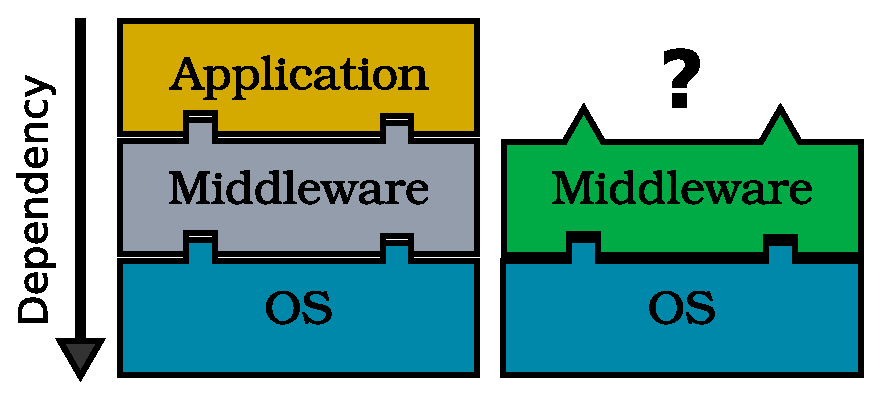
\includegraphics[height=80pt]{graphics_tables/bad_layers.eps} 
\caption{Layered Architecture}
\label{fig:bad_layers}
\end{figure}

The problem with the earlier component framework is that they are based on a strictly layered approach, as illustrated in figure
\ref{fig:bad_layers}. Traditionally systems are structured in layers where the more abstract layers depend on more the concrete
layers below them. The benefit is that the higher level layers can be built without worrying about low-level concerns. The
drawback is that the higher level layers are tightly coupled to the layers directly below them and are usually not portable
to other stacks. This problem can be mitigated by creating standards for the API of a layer, like \texttt{POSIX}, but cannot
be completely eliminated. 

With inversion of control, the infra-structure can sometimes be abstracted away completely eliminating source dependencies
on infra-structure APIs. As will be explained in the chapter about \texttt{SCA}, dependency injection can be used to adapt
a generic component to a specific middleware platform, by introducing a layer that inverts the direction of dependencies,
as shown in figure \ref{fig:good_layers}.

\begin{figure}
\centering
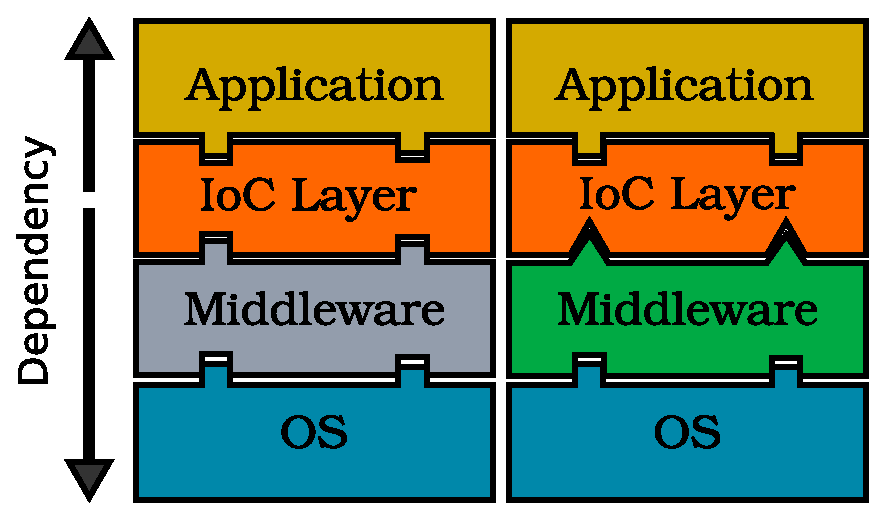
\includegraphics[height=80pt]{graphics_tables/good_layers.eps}
\caption{Inversion of dependencies}
\label{fig:good_layers}
\end{figure}


\textbf{Interoperability} Component frameworks like CCM are created to foster the reuse of software components.
Unfortunately these component frameworks are incompatible: a component in a CCM container cannot use a COM
component directly. So the platforms created to enable reuse can actually hinder it in some situations, creating
islands of compatibility. 

There are several solutions to bridge the gap between different middleware platforms such as the translation of
network protocols. But it would be even better if the component framework to use was just a matter of external
configuration. Then we could take two components and configure the remote method invocation protocol they should
use to talk to each other.

  
\chapter{Reflection}
  \label{chap:reflection}
  % TODO: talvez seja uma boa usar as definicoes e termos do Lakos da secao 5.4

Every computational system is built to solve a particular problem. As a consequence, all data structures and procedures
of a program represent this particular problem domain. A reflective system is one that is augmented with a representation
of itself. In other words, a reflective program can perform computations about its own computation.

Self-reference is a deeply philosophical issue and is often identified as an essential property of intelligence. For instance,
in his highly influential book, \texttt{Gödel, Escher, Bach: An Eternal Golden Braid}, Hofstadter \cite{Hofstadter} discusses how
Gödel's incompleteness theorem, biological systems and human intelligence all exhibit forms of self-reference and
self-representation. As a result, it should come as no surprise that the first studies of computational reflection came
from the mathematical logic and artificial intelligence communities.

One of the earliest works in computational reflection was Smith's \texttt{3-LISP} language \cite{Smith}, which he proposed as a first step towards
intelligent systems that could reason about themselves. Smith first considered the possibility of a self-referential language
when he wrote an interpreter for the KRL language in that same language. Later he refined his ideas in a new version of the
LISP language where the interpreter would expose details about the interpretation to the program being interpreted. In this language,
which he called \texttt{3-LISP}, an interpreted program could manipulate its own expressions, continuations and environments, thereby
changing its own behavior.

One aspect of self-reference is that it can go on indefinitely. An interpreter written in the same reflective language that it
interprets opens up the possibility of infinite levels of reflection, requiring what Smith called an infinite tower of interpreters.
In practice, this issue is solved by a so-called meta-circular interpreter that is able to simulate the infinite levels of regression.

Smith also outlined six general properties of reflective systems. The first principle is the requirement of a causal connection between
its self-representation and its behavior. This means that a reflective program should use this information to alter its
behavior. It would be useless if a process only contemplated itself without any further consequence. The second property is that
self-reference is necessarily associated to a theory, a representation of the knowledge, of itself. The third property is that
self-reference does not entail the ability of focusing on its current self. A process can only inspect what it was doing before
taking up the reflective activity. Otherwise, it could reflect about itself reflecting about itself reflecting ... and so on.
The fourth property of reflection is that it enables a finer grained control over the behavior of a program. In other words, it
enables more sophisticated programming techniques. The fifth property is that total detachment or objectivity is not possible,
because the self-knowledge is represented in the same formalism. The last property is that ``..Being reflective is a stronger
requirement on a calculus than simply being able to model the calculus in the calculus''. The ability to reflect cannot be
programmed from the inside. A Turing machine can simulate another Turing machine augmented with reflective capabilities but it
cannot reflect about itself. We will return to some of these points throughout this discussion.

The next step in the research of computational reflection was its application to object-oriented languages. In her seminal paper, Maes \cite{Maes}
outlined the basic features of reflection in an object-oriented context. The language \texttt{3-KRS}, built to demonstrate her ideas, had the
following properties:

\begin{enumerate}
 \item A split between object-level and meta-level. The meta-level was comprised of objects containing informations about the user-defined
object.
 \item A uniform self representation: everything in \texttt{3-KRS} is an object and consequently has a meta-object that can be inspected.
 \item A complete self-representation. Every object has a meta-object.
 \item Self-consistency. The meta-level is consistent with the object level and \emph{vice versa}. A modification to one entails a modification
to the other. 
  \item Modifiable self-representation. Meta-objects in \texttt{3-KRS} can be modified.
\end{enumerate}

This design has several interesting consequences. First of all, properties 2 and 3 guarantee that all entities in a program can be
inspected by the program itself. This alone opens up a myriad of possibilities of generic programming, auditing and debugging.
Second, properties 4 and 5 enable the modification of object properties at runtime since, to maintain consistency, modifications
in the meta-level must be reflected in the object level. Third, as a consequence of the uniformity property, the meta-objects themselves
have meta-objects that can be modified. An example of a modification is the addition, removal or redefinition of methods and attributes.

The same design was followed in the implementation of the Common Lisp Object System (CLOS) and its Meta Object Protocol (\texttt{MOP}) \cite{Kiczales}.
The idea behind CLOS, according to the authors, was to define a region in the design-space of programming languages instead of
a point. Because there are several ways to implement object-oriented mechanisms, each involving different trade-offs, CLOS was
designed to be adaptable to the needs of different application domains. To enable this, some basic mechanisms such as the
rules of method calls could be modified by specializing meta-classes.

Sadly, all this flexibility also introduces several new problems. One is that of meta-stability. In the words of Kiczales and colleagues,
the modification of objects at runtime could result in spectacular failure modes \cite{Kiczales}. Another serious issue is the performance price
that inevitably must be paid to compensate for the added flexibility. Taking this into account, the design of the \texttt{MOP} restricts
the possibilities of modifications in critical mechanisms, such as method dispatch to enable implementers to make optimizations.
For example, there are methods of meta-classes that are required to be idempotent. This allows the implementation to call
these methods only once and \emph{memoize} the result. However, even with these considerations there is anecdotal evidence
that suggests that opening the language for modification results in a performance overhead that is prohibitive for some applications \cite{Lee}.

Another problem is the runtime infra-structure needed for a self-modifiable program. So far in this discussion, it was implicit
that all discussed languages were interpreted rather than compiled. Even considering that everything is ultimately interpreted
by the underlying hardware, it would be a considerable challenge to implement the previously discussed kind of dynamism in
a compiled language. The language runtime would have to include a compiler. There are tools that can be used to provide
a meta-object protocol for compiled languages, but they are restricted to compilation or load time \cite{Chiba95} \cite{Chiba2000}.

Of course it is difficult to draw a line between compiled and interpreted languages. One reason, as mentioned, is that the hardware
itself is an interpreter. Another one is that, even interpreted languages, are usually parsed and compiled to a representation that is
easier to handle by the interpreter. A criteria that we can adopt is the following: in compiled languages, the interpreter, be it hardware
or software, cannot understand the source language, while in interpreted languages it does. This property of interpreted
languages is often made explicit by the presence of an \texttt{eval} primitive that can be called by the program at runtime
to interpret more code in the form of source text.

A further issue is that runtime modification of a program would be difficult to conciliate with static typing, which is the norm
in compiled languages. In languages with static typing, types are used as contracts between different parts of a program. 
These contracts enable the compiler to generate optimal code for method invocations because it knows precisely what argument
types to expect.

For the reasons mentioned above, reflection in compiled languages, if supported, is usually restricted to what is known
as introspection. This means that the meta-data can be inspected but not modified, what implies that no changes
have to be reflected back to the object level. However, somewhat ironically, in statically typed languages, this
limited form of reflection is much more useful than it would be in dynamic languages, because it enables the use of types
that were unknown at compile time. In other words, introspection can be used to simulate dynamic typing in a statically typed language.

The primary example of a statically typed language with native introspection is \texttt{Java}, so we will discuss its reflective features in detail
and use it as an inspiration for the implementation of an introspection support for \texttt{C++}. Finally, we wish to point out that reflection
is not an exclusive property of the programming language. Reflection is also possible at other abstraction layers, such as the architectural
level.


\section{Introspection in Java}

\texttt{Java} is a statically typed language that is compiled to the bytecode of the \texttt{Java} Virtual Machine (\texttt{JVM}). The fact that it is not executed
directly by hardware does not mean that it can be seen as an interpreted language: there is no \textbf{eval} primitive.
The reason for analyzing \texttt{Java} in detail in this discussion is that \texttt{Java} has a native introspection support and has many
similarities with \texttt{C++}.

Each source file of \texttt{Java} contains the definition of a single class and is compiled to a bytecode file called a class file.
Class files have a dual role in \texttt{Java}. The first role corresponds to that of header files in \texttt{C++}: the
declaration of types and methods used by other compilation units. The second second role corresponds roughly to that of
\texttt{C++} object files, containing data to direct the linkage of compilation units. This dual use forces this file format to
preserve information about classes, such as the the number and signature of methods, attributes and constructors.
Furthermore, compilation units in \texttt{Java} are linked at runtime when they are loaded into the \texttt{JVM}. Given that
class meta-data is present when classes are loaded, it is only logical to make it available to the programmer by means
of an introspection API instead of discarding it after linking. Another interesting feature of \texttt{Java} is that the loading
of classes can be customized. Application programmers can provide their own custom class loaders, which presents the
opportunity to modify classes before they are linked, enabling a meta-object protocol at load time \cite{Chiba2000}.

Having seen how class meta-data is obtained by the \texttt{JVM}, let us now turn our attention to the architecture of the
introspection \texttt{API}. In \texttt{Java}, every class is associated to a meta-object of the class \texttt{java.lang.Class} and every object
inherits from the base class \texttt{java.lang.Object}. The \texttt{Object} base class can be used to obtain a reference to the meta-object of
its class. Only single inheritance of implementation is possible in \texttt{Java} so this reference always points unambiguously to the
meta-object of the most concrete class of an object. Observe that, because in \texttt{Java} classes are not first-class citizens, they
cannot be collapsed with their meta-objects as is the case in prototype-based object-oriented languages.

The class \texttt{java.lang.Class} has class-global methods to search classes by name and to list all classes, so the meta-data for all
classes is reachable at runtime. The information made available by an instance of \texttt{java.lang.Class} basically consists of the
class's visibility, a list of its constructors, a list of its attributes and a list of its methods. These lists include not only
\texttt{public} entities but also those with \texttt{protected}, \texttt{private} or \texttt{package} visibility, making it
possible to bypass the access restrictions.

The entities accessible through a class meta-object are meta-objects as well. Attribute meta-objects are instances of the class
\texttt{java.lang.reflect.Field}, constructors and methods are represented by the classes \texttt{java.lang.reflect.Constructor} and \texttt{java.lang.reflect.Method}
respectively. There is no need to go into much detail here so we will only present a brief summary of the functionality provided
by theses classes.

The \texttt{Field} meta-object can be used to inspect the name and the type of an attribute. The type information is given in the form of
a reference to a Class meta-object. In addition, this object can be used to obtain and to change the value of the given attribute in
a specific object. The value is returned using a reference to the universal base class, \texttt{Object}. A minor difficulty arises due to the
fact that primitive types are not objects in \texttt{Java}. To deal with this, for each primitive type \texttt{Java} defines a container class such
as \texttt{java.lang.Integer} and seamlessly performs \emph{auto-boxing} when necessary.

Constructor meta-objects provide information about the number of arguments in addition to the type of each one of them. Constructor
objects also have a method that takes an array of Objects calls the reified constructor passing these arguments, and returns a new
instance of the class this meta-object is associated with. The class meta-object has a shortcut method called \texttt{newInstance}
that finds a constructor based on the types of its arguments and uses it to return a new object.

Finally, \texttt{Method} meta-objects are used to reify methods. They provide the methods name together with all the information relevant to
its signature: the return type, the number of arguments, and their types. As is the case with the \texttt{Constructor} class, the \texttt{Method}
class has a method to invoke the reified method. It takes as arguments a reference to the target object and an array of references
to \texttt{Object} representing the arguments and subsequently performs the call returning the result as an \texttt{Object}.

At first sight, this may seem as an overly complicated way of performing the usual operations on objects, but it enables many
advanced programming techniques that otherwise would be impossible because the reflected entities are not first-class citizens
of the language. Because of its static typing, in \texttt{Java}, the full definition of a class must be available at
compile-time whenever it is used. However, using introspection meta-classes, it is possible to interact with classes that
were unknown at compile-time. It also enables a style of programming generally known as \emph{duck typing}. Suppose that
we are building a system that draws objects on screen. The traditional static typing approach
would require that all graphic objects implement a common interface that declares a \texttt{draw} method. In contrast, with
\emph{duck typing} we simply check if the object has a method with an appropriate signature without bothering if the class
implements a specific interface.

It is also common to use introspection for meta-programming. Building on the previous example, suppose that we decide that
requiring the objects that are to be displayed to have a draw method is a bad design decision: it is difficult to specify
alternative forms of drawing and we may want to reuse these objects in contexts where they are not displayed. A draw method
inevitable makes use of a graphic library and we would be forced to include it even if it's not needed. A possible
approach is to define another hierarchy of objects to draw them. Listing \ref{lst:game1} shows the example of a computer game.
In many games, the enemies that the player has to defeat are assigned to different categories based on difficulty. Depending
on the current setting, the enemies might be of different species, but behind the scenes share the same artificial intelligence,
differing only in their appearance.

\begin{listing}[H]
\begin{minted}[linenos,fontsize=\footnotesize]{java}
public class DrawOrc implements DrawEnemy {

  public void draw(Enemy enemy) {
    
    if (enemy instanceof Soldier) {
      OrcSoldier.draw(enemy);
    } else if (enemy instanceof Captain) {
      OrcCaptain.draw(enemy);
    } else if (enemy instanceof Boss) {
      OrcBoss.draw(enemy);
    }
  }
} 
\end{minted}
\caption{Example of a code with unecessary repetition}
\label{lst:game1}
\end{listing}

There clearly is a pattern in the code of Listing \ref{lst:game1}: for each class there is another class with a predictable name. With introspection we
can automate all this tedious typing, as shown in Listing \ref{lst:game2}

\begin{listing}[H]
\begin{minted}[linenos,fontsize=\footnotesize]{java}
public class DrawOrc implements DrawEnemy {

  public void draw(Enemy enemy) {
    Class c = enemy.getClass();    
    Class d = Class.forName("Orc" + c.getSimpleName());    
    Method draw = d.getMethod("draw", Enemy.class);
    draw.invoke(enemy);
  }
}
\end{minted}
\caption{Example of meta-programming based on introspection}
\label{lst:game2}
\end{listing}

Not only is this code more generic, but it also automatically handles new cases. It can even handle new cases at runtime: we could load
the classes \texttt{Warrior} and \texttt{OrcWarrior} and this code would automatically handle them. And there are even more possibilities
of meta-programming. We can load the drawing dispatcher class based on the name of the type of enemy of the current level. For example,
if the current type of enemy is ``\texttt{Alien}'' we could load the class \texttt{DrawAlien} by name.

Another interesting feature of \texttt{Java}'s introspection support is what is called \texttt{dynamic proxies}.
In object-oriented programming, the \emph{proxy design pattern} \cite{Gamma} is a way of intercepting the method
invocations to an object. This is done by inserting a \emph{proxy object} between the target and client objects.
For this to be possible, the target object must be substitutable for the proxy objects. In languages like \texttt{Java}
and \texttt{C++}, this is achieved by making the proxy object implement the same interface as the client object. 
A proxy class can be hand written for a specific case and compiled together with the application. However the
standard introspection library in \texttt{Java} allows one to create proxies at runtime for one or more interfaces.
In \texttt{Java}, interfaces are special classes comprised only of the signature of methods. These interfaces are used
to specify contract between objects and more than one of them can be inherited, or in \texttt{Java} parlance,
\emph{implemented} by standard classes. Dynamic proxies enable the programmer to implement interfaces during
the execution of the program. The method invocations on those interfaces are intercepted 
by the dynamic proxy and then the arguments are inserted in an array of parameters and forwarded to a handler object specified
by the programmer. This feature has many applications that would otherwise be difficult to achieve without explicitly generating
source code for each implemented interface. Consider, for example, the implementation of remote invocation stubs. Upon receiving
a method call, the stub must find out which method was called, put this information together with a serialized representation
of the arguments in a packet, and send it across the network. Without dynamic proxies, the programmer would have to use
a tool to read the definitions of interfaces and generate a stub source file for each one, every method containing slightly
different code to handle the method's signature.

To illustrate this concept, consider again the computer game example. As previously noted, the implementation of the drawing dispatchers
is quite mechanical. With dynamic proxies, we can automate the definition of these classes, as shown in Listing \ref{lst:game3}

\begin{listing}[H]
\begin{minted}[linenos,fontsize=\footnotesize]{java}

public class DrawingDispatcher 
  implements java.lang.reflect.InvocationHandler {
  
  private String enemyType;
  
  public Object invoke(Object proxy, Method m, Object[] args)
	throws Throwable
    {
	Enemy enemy = (Enemy)args[0];
	Class c = enemy.getClass();    
	Class d = Class.forName(this.enemyType + c.getSimpleName());    
	Method draw = d.getMethod("draw", Enemy.class);
	
	return draw.invoke(enemy);
    }
}

public class Game {

  public static void main {
  
    DrawEnemy drawOrcs = (DrawEnemy)
      java.lang.reflect.Proxy.newProxyInstance(
	DrawEnemy.class.getClassLoader(),
	new Class[] { DrawEnemy.class },
	new DrawingDispatcher("Orc"));
					
    DrawEnemy drawAliens = (DrawEnemy)
      java.lang.reflect.Proxy.newProxyInstance(
	DrawEnemy.class.getClassLoader(),
	new Class[] { DrawEnemy.class },
	new DrawingDispatcher("Alien"));
    
  }
}
\end{minted}
\caption{Example of dynamic proxies in Java}
\label{lst:game3}
\end{listing}

Hassoun and colleagues interpret \texttt{Java's} dynamic proxies as the meta-objects of \texttt{CLOS}' meta-object protocol, but
we think this is an overstatement, since the possibilities of dynamic proxies are limited to intercepting method calls, and
they require programmers to follow the rule of separating interface from implementation, whereas meta-objects can
be used to change the behavior of any object \cite{Hassoun03, Hassoun05}. 

The separation of interface and implementation is essential for achieving Martin's \texttt{Open-Closed Principle} that states
that object-oriented designs should strive to be closed for modifications but open for extensions. Dynamic proxies can
be used very effectively to extend and configure existing designs at runtime, when interfaces are separated from implementation.
Several cross-cutting concerns can be handled with proxies. For example, the \texttt{Spring Framework for Java} provides a
proxy implementation that wraps method call in database transaction transparently.

To conclude this overview of reflection in \texttt{Java}, we point out that it arguably conforms to the first four requirements listed by
Maes \cite{Maes}. Not all entities are objects as required, but all have meta-objects.

\section{Introspection in C++}

\texttt{C++} is a superset of C that supports object-oriented programming. The design of \texttt{C++} is primarily concerned with the most efficient
implementation of abstractions. Also, the design is guided by the principle that the programmer should only pay for what
is effectively used (the currency being \texttt{CPU} and memory overhead). So, for instance, polymorphism is not enabled by default
for objects, one has to explicitly mark at least one method as \emph{virtual} to obtain this behavior.

In \texttt{C++}, introspection is severely limited. Basically, all that can be done at runtime is comparing types for equality. Most likely, a complete
introspection support was never introduced because it is difficult to conciliate the inherent space overhead with the ``pay only for what
is used'' approach. At compile-time, template meta-programming techniques can be used to obtain information about classes.
In particular, a technique called Substitution Failure Is Not An Error (SFINAE) can be used to detect if a class has a method with
a specific name and signature. Combining compile-time introspection with runtime introspection, it is possible to obtain more
detailed runtime information. However, these techniques can only answer yes-no questions like ``Is class A derived from class B?''.
There is no way, for example, to enumerate all methods of an object.

Clearly, this situation is far from satisfactory and several introspection extensions have been proposed, but most stumble upon
two primary difficulties. In \texttt{C++}, as specified in the \texttt{ISO} standard of 1998, there is no way of referring to generic entities 
without losing all type information. In \texttt{Java}, every objects can be referred to using the universal \texttt{java.lang.Object} base class
and as we have seen, this base class can be used to recover the full type information of an object. In \texttt{C++}, there is the \texttt{void*}
pointer that can point to anything, but unfortunately the already limited introspection facilities of the language cannot interact
with this kind of pointer, so the type information cannot be recovered. Another difficulty is that, in this version of the standard,
it is impossible to declare methods that accept a variable number of arguments. This makes the implementation of a totally generic
\texttt{Method} meta-class impossible.

To introduce more advanced introspection in \texttt{C++} two main issues must be addressed:

\begin{enumerate}
 \item \textbf{Compilation of meta-data}. All the information about types definitions, methods and functions must be obtained in a way that
is compatible with standard \texttt{C++} implementations.
 \item \textbf{Presentation of meta-data}. \texttt{C++} is a very convoluted language with many special cases. This makes it difficult to
 present a consistent and general view of the meta-data. Also, if runtime introspection is to be supported, the interactions
 with types unknown at compile-time must be carefully designed to be usable.
\end{enumerate}

Attempts to introduce reflection in \texttt{C++} were made almost since the language was created. For example, in 1995 Chiba \cite{Chiba95} proposed
a meta-object protocol for \texttt{C++}, but it was limited to modifications at compile-time. 

Perhaps the most widely known implementation of introspection support for \texttt{C++} is the \texttt{SEAL} \cite{seal} library developed at \texttt{CERN}. It is very
detailed, including meta-data for \emph{typedefs}, scopes, primitives and arrays. It has a method call construct, but it is not type-safe,
as arguments are passed as an array of void pointers and, consequently, unsafe type conversions must be used on the receiving side.
It uses a parser that generates meta-data and method call code in \texttt{C++} that must be compiled and linked to the program that uses it.

Chuang and colleagues \cite{Chuang} describe an introspection system for \texttt{C++} that aims at being non-intrusive and that supports
loading of new classes and meta-data at runtime. However, they make extensive use of \texttt{void*} pointers leading to unsafe type
conversions.

Devadithya and colleagues \cite{Devadithya} present a reflection system similar to \texttt{SEAL}. It uses template classes to hold method pointers
and do the calls. The number of of arguments is limited to the number of template specializations implemented in the library.
The exact argument and return types must be known, which has as consequence that the end user code needs their complete
definitions. 

\texttt{Reflection for C++} \cite{garret} proposes the gathering of meta-data out of debug information generated by compilers.
This has the advantage that the meta-data can be extracted of executable files. The drawback is that the code must be compiled
in debug mode. To further complicate matters, each compiler uses a different representation for debug information.
In addition, this proposal requires modifications of reflected classes, denying the possibility of introspecting existing code.

The \texttt{Rich Pointer} proposal \cite{RichPointers} proposes a special kind of generic pointer that, in contrast to \texttt{void*}, would
not loose the runtime type information associated with the referenced object. These pointers could be cast to normal pointers,
allowing their use with legacy code. In addition, this work proposes a comprehensive runtime type information system that would
enable the iteration over the set of methods of a class, for example. At the time of this writing, the authors of the proposal express
the intention of adding a construct to call methods and functions dynamically, but no further details are given.

There are proposals to add compile-time introspection to \texttt{C++} in a form suitable for template meta-programming \cite{Chochlik}.
Compile-time and runtime introspection address slightly different concerns and present different trade-offs. Compile-time
introspection could advance compile-time meta-programming beyond what is possible today with template meta-programming techniques.
For example, it could be used to generate object-relational mappings to store objects in a relational database.
In addition, the compiler would have many opportunities for optimization. Because every use of meta-data is known, the compiler
can discard unused data, reducing the memory overhead. Runtime method calls using pre-compiled introspection mechanisms could
also be optimized, the compiler knowing all variables involved. On the other hand, compile-time reflection cannot be used to
enable late binding. It would be impossible, for example, to load a module during the execution of a program and
use the classes defined in it.

And finally, there are approaches that modify the language itself. For example, Microsoft supports an extended \texttt{C++} for their
Common Language Runtime (CLR), which provides reflection for all supported languages, including \texttt{C++} \cite{CLR}. Another notable
example is the \texttt{Qt} framework. It provides a mechanism called \emph{signals and slots} that enables a restricted form
of late binding that makes it possible to connect objects at runtime without requiring their definitions to be available during compilation of either parts.
However, \texttt{Qt} requires the extension of the language with additional keywords and forces all connectable objects to inherit a common base class, which introduces
difficulties when multiple inheritance is needed. 

Not directly related, but still relevant is \texttt{CERN}'s \texttt{C++} interpreter, \texttt{cling} \cite{cling}, that uses the \texttt{clang}
\cite{cling} compiler and \texttt{LLVM}'s infrastructure to dynamically compile \texttt{C++} code. In view of the above discussion of the relation between
interpretation and reflection, this could open interesting possibilities.

\subsection{Existing introspective features of C++}

\texttt{C++} is not totally devoid of introspection. There are some very limited introspective features both at compile-time and
at runtime. In the following section, we will analyze them in detail not only for the purpose of comparison but also because
our proposed introspection extension is partly built using these features.

\subsubsection{Runtime type introspection}

\texttt{C++} provides some forms of runtime introspection, collectively known as runtime type information (\texttt{rtti}). The most commonly
used \texttt{rtti} operation is the \texttt{dynamic\_cast} that permits the programmer to navigate in a class hierarchy.
The \texttt{dynamic\_cast} can be seen as a built-in function template which takes a pointer to a polymorphic object and a destination type
as template parameter. It thus takes two types as parameters: the origin type implicitly specified by the pointer argument, and the
explicitly specified destination type. If the object referred to by the argument pointer is an instance of the requested class, a pointer of
the correct type, pointing to that same object, is returned. Otherwise, a null pointer is returned. Therefore the \texttt{dynamic\_cast}
enables us to ask if the object pointed to is an instance of the destination type, with the restriction that both types must be in the same
hierarchy of polymorphic classes. There are two restrictions on origin and destination that severely limit the functionality of the
\texttt{dynamic\_cast}: both must be polymorphic types, and both must be in the same class hierarchy. The first restriction excludes not
only classes without virtual methods but also primitive types. In particular, the \texttt{void*} pointer cannot be used, eliminating
the possibility of using the dynamic cast as a general \texttt{instanceof} operator as in \texttt{Java}. If the second restriction were lifted,
we could at least use this operator to introspect all polymorphic classes but, unfortunately, this is not the case. A more subtle limitation
of this operator is that the declaration of both types must be visible at the same source location where it is used.

Another form of \texttt{rtti} is the \texttt{typeid} operator. This operator returns a reference to an object of the standard class
\texttt{type\_info}. Basically, the only thing that can be done with this object is to compare it for equality with other objects of
this class. The standard library defines a special \texttt{operator==} to compare two references to \texttt{type\_info}. If this
comparison operator returns true, both \texttt{type\_infos} refer to the same type. The \texttt{typeid} operator is applicable to all
types, making it possible to formulate expressions like \verb|typeid(double) == typeid(std::string)|. In addition to its universal
applicability, this operator also gives us an opaque reference to type-dependent information. It is possible to compare
\texttt{type\_info} object even if the types they represent are not known at compile type. The greatest disadvantage of this
operator is that it is agnostic to class hierarchies. For this reason, \verb|typeid(A) == typeid(B)| evaluates to false even if
\texttt{B} inherits \texttt{A}. Most of the functionality of this operator can be simulated using \texttt{templates} that implement
a polymorphic base class with a custom equality operator that internally performs a \texttt{dynamic\_cast}, as demonstrated in
Listing \ref{lst:typeid}. The reverse is not possible.

\begin{listing}[H]
\begin{minted}[linenos,fontsize=\footnotesize]{c++}
 
struct sim_type_info {
  virtual bool operator==(const sim_type_info& other) const = 0;
};

template<typename T>
struct sim_type_info_impl: public sim_type_info {
  bool operator==(const sim_type_info& other) const {
      return dynamic_cast<const sim_type_info_impl*>(&other) != 0;
  }
};

template<typename T>
const sim_type_info& sim_typeid() {
  static sim_type_info_impl<T> inst;
  return inst;
}  

template<typename T>
const sim_type_info& sim_typeid(const T& exprResult) {
  return sim_typeid<T>();
}
\end{minted}
\caption{Simulating typeid with templates and dynamic\_cast}
\label{lst:typeid}
\end{listing}

The last form of \texttt{rtti} is never mentioned in \texttt{C++} programming manuals, which is surprising, as it is really the most powerful one.
Because in \texttt{C++} any value, object or reference can be used as operand of the \texttt{throw} operator, the exception handling
machinery must include the type information of the thrown entity to guarantee that the correct catch statement is called.
Listing \ref{lst:dyncast} shows how a \texttt{dynamic\_cast} operator can be implemented with exception handling.

\begin{listing}[H]
\begin{minted}[linenos,fontsize=\footnotesize]{c++}
template<typename Orig, typename Dest>
Dest* dyn_cast(Orig* o) {
  try {
      throw o;
  } catch (Dest* d) {
      return d;
  } catch (...) {
      return nullptr;
  }
}
\end{minted}
\caption{A cast implementation using exception handling}
\label{lst:dyncast}
\end{listing}

Actually, the above \texttt{dyn\_cast} in some aspects is more powerful than the \texttt{dynamic\_cast} because \texttt{Orig} and
\texttt{Dest} do not need to be in an inheritance relation, they can even be primitive types. Not all traversals of an inheritance
hierarchy graph are supported but the conversion of a more concrete type to a more abstract type is guaranteed to work.
Of course, this is an abuse of exception handling for a totally different purpose, so we cannot expect it to be as efficient
as the other forms of \texttt{rtti}. The advantage of this mechanism is that the code that throws can be defined in one translation unit
and the catching code in another. Better yet is the fact that the catching code does not need the declaration of type that is effectively
thrown and, conversely, the throwing code does not need to know the types that appear in the catch statement. 

Before we continue with the next topic, we wish to point out that the examples in this section not only demonstrate the relationship
between the different forms of runtime introspection in \texttt{C++}, but also illustrate the interesting interactions with templates, a compile-time
feature.

\subsubsection{Compile-time introspection}

Compile time introspection in \texttt{C++} is a side-effect of templates. Templates are a form to declare classes and functions that are parameterized
by types or integer constants. This makes it possible, for example, to write a linked list data structure for any type without resorting
to \texttt{void*} pointers as is common in \texttt{C}. With the intention of allowing reusable data structures and algorithms, the designers
of \texttt{C++} introduced a Turing-complete compile-time language. This has originated a number of interesting techniques called template
meta-programming, that were exploited to generate optimal linear algebra code\cite{veldhuizen}, create concrete products out of product
lines\cite{Czarnecki98} and implement object-oriented design patterns efficiently \cite{Alexandrescu1}. The introduction of templates that accept
a variable number of arguments in \texttt{C++11}, known as \emph{variadic templates}, has greatly improved the programming style for an unknown number
of arguments.

The basis for template meta-programming is template specialization that can be used as a compile-time \emph{if-then-else} statement, as seen in Listing \ref{lst:staticif}

%\begin{minipage}[b]{0.45\linewidth}
%\centering
\begin{listing}[H]
\begin{minted}[linenos,fontsize=\footnotesize]{c++}
template<bool B, typename U, typename V>
struct Select {
	typedef V type;
};

template<typename U, typename V>
struct Select<true, U, V>
{
	typedef U type;
};
\end{minted}
\caption{Static if-then-else}
\label{lst:staticif}
\end{listing}
%\end{minipage}
%\begin{minipage}[b]{0.55\linewidth}
%\centering
\begin{listing}[H]
\begin{minted}[linenos,fontsize=\footnotesize]{c++}
template<int N>
struct fact {
  enum { value = N*fact<N-1>::value };
}

template<>
struct fact<0> {
  enum { value = 1 };
}
\end{minted}
\caption{Static recursion}
\label{lst:staticrec}
\end{listing}
%\end{minipage}

And since integer constants may be used as template arguments, we have recursion as well, as shown in Listing \ref{lst:staticrec}
The most impressive consequence of template specialization, however, is the compile-time introspection that results. For example,
Listing \ref{lst:templintros1} shows how we can determine if a given type is a pointer using specialization.

\begin{listing}[H]
\begin{minted}[linenos,fontsize=\footnotesize]{c++}
template<class T>
struct is_a_pointer {
  enum { value = false };
}

template<class T>
struct is_a_pointer<T*> {
  enum { value = true };
}
\end{minted}
\caption{Compile-time introspection}
\label{lst:templintros1}
\end{listing}

An even more impressive use of templates is a technique called Substitution Failure Is Not An Error (SFINAE).
The code in Listing \ref{lst:sfinae} employs this technique to test if a type supports the equality operator.

\begin{listing}[H]
\begin{minted}[linenos,fontsize=\footnotesize]{c++}
namespace comparable_impl {

  typedef char no;
  typedef char yes[2];

  template<class T>
  no operator==( T const&, T const& );

  yes& test_eq( bool );
  no test_eq( no );

  template<typename T>
  struct test {
    static T const& t1;
    static T const& t2;
    static bool const value = sizeof( test_eq(t1 == t2) ) == sizeof( yes );
  };

}

template<typename T>
struct comparable {
  enum { value = comparable_impl::test<T>::value };
};
\end{minted}
\caption{SFINAE: Determine if a type supports comparison}
\label{lst:sfinae}
\end{listing}

In generic programming it is often the case that a type template parameter does not provide enough information for
the implementation of a data structure of algorithm. In these cases it is common practice to use as argument \texttt{structs}
that contain additional information in the form of \texttt{typedefs} and integer constant definitions. These \texttt{structs}
are known as \emph{type traits}, their most prominent use being the standard \texttt{std::string} class that is actually
a template instantiation that takes as argument a \texttt{char\_traits<char>}. Due to the widespread use of traits, the \texttt{C++11}
standard introduced a new standard header file, \texttt{<type\_traits>} that contains useful templates such as
\verb|std::is_arithmetic<T>| and many others that provide a lot of introspective information for generic template programming.

Needless to say, because it was not their original purpose, meta-programming with templates is unwieldy and requires
a lot of trickery. But the greatest limitation of these techniques is that they can only answer yes-no questions about types.
There is no way to iterate over the existing types and list their methods and attributes. 

\section{The SelfPortrait extension}

We have designed a runtime introspection extension for \texttt{C++11} called \texttt{SelfPortrait}. We chose this name because a self-portrait
is a necessarily simplified representation of oneself. Also, a painting is meant only for contemplation but not for modification. In
the same spirit, this extension provides an abstract representation of \texttt{C++}, in \texttt{C++}, but has no complete meta-object protocol that would
allow runtime modification of a program. It is an extension in the sense that the compilation model is extended, although no proper
language modification is required.

As advocated by Maes \cite{Maes} and followed in previous approaches, our extension provides a meta-model layer that is strictly
separate from the application domain model. The skeleton of our meta-model is basically the same as \texttt{Java}'s but was adapted to
\texttt{C++}'s characteristics where needed. In comparison to the meta-models of previous introspection proposals for \texttt{C++}, such as \texttt{SEAL} reflex \cite{seal},
ours is somewhat simpler because we are only concerned with the introspection of runtime entities.

What distinguishes the \texttt{SelfPortrait} extension from previous works is that we address the following key issues:

\begin{enumerate}
 \item Opaque and uniform handling of types without loss of type information
 \item Function, method and constructor invocations without restriction on the number and types of arguments
 \item Dynamic proxies
\end{enumerate}

Opaque handling of types goes hand-in-hand with generic function invocations as it allows to manipulate arguments and return
values of unknown types. The unrestricted invocation of functions through introspection is an essential feature without which
the applicability of introspection is limited to a few special cases. And finally, as argued in our survey of \texttt{Java}'s introspection,
dynamic proxies are a very powerful construct that can be used for the transparent interception of method calls or for mechanical
implementations of interfaces. 

Our implementation is guided by the following requirements:

\begin{enumerate}
 \item All type conversions should be checked at runtime, there should be no conversions to and from \texttt{void*}.
 \item No changes should required of introspected code. We must not impose the inheritance of a common base class to introspected classes.
 \item The usage of meta-classes should be as natural as possible. Where needed we should add \emph{syntactic sugar} to help the programmer.
 \item It should be portable to any \texttt{C++11} conforming compiler.
\end{enumerate}

In the remainder of this section we will first present how we want the introspection \texttt{API} to look like and then explain
how this goal is attained.

\subsection{Proposed reflection API}
\label{proposed}

In short, we want the programmer to be able to perform the following operations:
\begin{enumerate}
 \item Listing of reflected classes and functions
 \item Listing of the relevant characteristics of classes: accessible attributes, methods, constructors and super classes
 \item Invocation of functions, methods and constructors.
 \item Handling of types whose declarations were not available at compile-time
 \item Dynamic implementation of interfaces
\end{enumerate}

In Listing \ref{lst:listing1} we present a simplified view of the \texttt{API} we want to implement. We have omitted many methods and the classes for
attributes and functions, but the essential parts are there. Basically, the user can obtain a \texttt{Class} meta-data object by name (line 7) and,
from there, locate its methods and attributes. The \texttt{Method} class at line 11 gives basic informations about the corresponding method including
name, number of parameters and their types, among other features. The sequences of three dots are part of \texttt{C++11's} notation for templates that
accept an unknown number of arguments.

The \texttt{VariantValue} type that appears in their signature is the opaque wrapper class for unknown types that will be described in section \ref{sec:variant}.
The template method \texttt{call} is only provided as syntactic sugar that captures the arguments, wraps them in variants and
calls \texttt{callArgArray}.

\begin{listing}[H]
\begin{minted}[linenos,fontsize=\footnotesize]{c++}
class Class {
  string name();
  Class superclasses();
  MethodList methods();
  AttributesList attributes();
  ConstructorList constructors();
  static Class forName(string name);
  bool isInterface();
};

class Method {
  string name();
  string returnTypeSpelling();
  list<string> returnArgumentSpellings();
  
  template<class... Args>
  VariantValue call(VariantValue& object, Args... args) { /*impl*/ }
  VariantValue callArgArray(VariantValue& object, vector<VariantValue>& args);
};
\end{minted}
\caption{The simplified interface for Class and Method introspection objects}
\label{lst:listing1}
\end{listing}

Instead of showing the \texttt{API} for dynamic proxies, Listing \ref{lst:proxies} shows an example
usage because it might not be immediately apparent how these are used from the \texttt{API} alone.
In line 1, we obtain a meta-object for a class called ``Foo''. Then, in line 3, we search for a
method named ``method1''. After that, we instantiate a proxy object, in line 5, passing the class
meta-object as argument. Proxies can be constructed for one or more classes. The only restriction is
that these classes should be \emph{interfaces}. We will explain this concept later in this section.
Then, in line 7, we add an implementation for a method in the form of a \texttt{C++11} lambda, but functions
and any object with an \texttt{operator()} can be used as well. To specify for which method we are
providing an implementation, we use the method meta-object that was retrieved earlier.
Finally, the remainder of this listing shows how we can obtain a reference to the implemented object
using the specified base class.

\begin{listing}
\begin{minted}[linenos,fontsize=\footnotesize]{c++}
Class foo = Class::lookup("Foo");

Method m = foo.findMethod([](const Method& m){ return m.name() == "method1"; });

Proxy proxy(foo);

proxy.addImplementation(m, [](const std::vector<VariantValue>& args){
  int first = args[0].value<int>();
  int second = args[1].value<int>();
  return VariantValue(first*second);
});

VariantValue handle = proxy.reference(foo);

Foo& stub = handle.convertTo<Foo&>();

int result = stub.method1(3,5);
\end{minted}
\caption{A sample usage of proxies}
\label{lst:proxies}
\end{listing}

Because we want the \texttt{API} to be as natural and as easy to use as possible for \texttt{C++} programmers,
we want the arguments to be converted implicitly and safely to the types that the method requires.
For example, if a parameter is passed by reference we want to get a reference to the value passed as argument.
On the other hand, if the parameter is passed by value we want a copy of the value. The best place to implement
these conversion is the \texttt{VariantValue} class. We can see some of the conversions that we would like to
support in Listing \ref{lst:listing5}.

\begin{listing}[H]
\begin{minted}[linenos,fontsize=\footnotesize]{c++}
VariantValue v("5"); // initialize
std::string s = v.convertTo<std::string>(); // copy
std::string& sr = v.convertTo<std::string&>(); // get reference
std::string* sp = v.convertTo<std::string*>(); // get pointer
int n = v.convertTo<int>(); // convert to to integer
\end{minted}
\caption{Requirements for VariantValue}
\label{lst:listing5}
\end{listing}


\subsection{Opaque handling of types}
\label{sec:variant}

Perhaps the most important feature of an introspection library for a statically typed language is to support the invocation
of methods without requiring their definitions to be available at compile-time. As in \texttt{Java}, this functionality is supplied by adding
a special method to the Method meta-object that forwards its arguments to the method that this object represents.
Because of the language's static typing, we can define this method only once and this definition must work with all possible method
signatures. This entails that the formal parameters of this generic method must be able to bind to all possible types.
In previous introspection proposals this was handled using arrays of \texttt{void*} pointers because. This approach presents several
serious problems. First of all, the conversion to \texttt{void*} pointer inevitably leads to a complete loss of type informations,
so the implementation of the generic call for a specific method has no choice other than blindly casting this pointer to one
of the desired type. If the user by mistake passed a pointer to an object of another type there will be no way of detecting this
situation and all kinds of memory corruption could follow. The second problem is that of usability. Because it is not possible
to take the address of a temporary, all arguments must be explicitly allocated on the stack or on the heap. Furthermore, in \texttt{C++}
if we pass an integer to a function that expects a double, the compiler will make the conversion without complaining. Using
\texttt{void*} pointers the programmer cannot simply pass the address of an int to a function that expects a double, because
this would lead to an erroneous memory access. In addition, with raw pointers in \texttt{C++} it is often difficult to decide who should
free the pointee if it was dynamically allocated.

What is required is an opaque handle that hides all type information but makes it possible to verify if the hidden type correspond to an
expected type and to extract the hidden value using this type. To fulfill this requirement we can use a special type of container
commonly known as \emph{variant}.

Variants are like \texttt{void*} pointers enhanced with type information and life-cycle management.
Most variants are implemented either using unions, as described by Alexandrescu\cite{Alexandrescu2}, or usings template class implementing
an abstract interface, a technique called \emph{type erasure} \cite{Becker} described by Henney\cite{Henney}. boost::any and boost::variant\cite{boost}
are good examples of both alternatives. The problem of the union approach is that the variant is restricted to a finite set of types, so our variant
implementation follows the type erasure approach due to its greater flexibility. The improvement of our variant over existing implementations
is that even types without default or copy constructor can be used. Indeed, any constructor can be used. In addition to values, our variant
can also contain references, a capability that is essential to avoid the introduction of copies when a parameter is passed by reference.
The object held can be accessed by copy, by reference or by pointer. Most importantly objects can be accessed by references and pointers to
base classes. Additionally, it is detected at compile time if the type is convertible to std::string or arithmetic types. If this is the
case, conversions to any arithmetic type or std::string are automatically implemented. The arithmetic type conversion is very convenient
because it allows us to pass a variant containing a char where an int is expected, just like the compiler would accept for temporary values.
The philosophy of our variant in this respect is like Qt's QVariant's\cite{qt}: what matters most is not the real type hidden inside the
variant, but the types it can be converted to. This frees us from painstakingly constructing variants of an exact type.

\begin{listing}[H]
\begin{minted}[linenos,fontsize=\footnotesize]{c++}
class VariantValue
  unique_ptr<IValueHolder> m_impl;
  
  template<class ValueType>
  typename normalize_type<ValueType>::ptr_type 
  isA_priv() const {
    try {
      m_impl->throwCast();
    } catch(typename normalize_type<ValueType>::ptr_type ptr) {
      return ptr;
    } catch (...) {
      return nullptr;
    }
  }
  
public:
  template<class ValueType>
  ValueType value() const {
    auto ptr = isA_priv< ValueType >();
    if (ptr == nullptr) {
	// throw (error handling omitted)
    }
    return *ptr;
  }
  // other methods...
};

template<class ValueType>
class ValueHolder: public IValueHolder {
  ValueHolder m_value;
public:
  virtual void throwCast() const {
    throw &m_value;
  }
private:	
};
\end{minted}
\caption{Conversion of variants}
\label{lst:listing11}
\end{listing}

In Listing \ref{lst:listing11} we can see the essential aspects of our Variant implementation. We have a front-end called \texttt{VariantValue} (line 1)
with value-semantics that holds a pointer to the abstract base class \texttt{IValueHolder} which in turn is implemented by the class template
\texttt{ValueHolder} (line 28). (The abstract base class has been omitted to avoid redundancy)

As the reader might have noticed we use the flexibility of the \texttt{rtti} functionalities derived from exception handling.
At line 33 in method \texttt{throwCast}, where the type of the contained value is known, we throw a pointer to it. At line 8
we call the \texttt{throwCast} method and an line 9 we try to catch a pointer to a type provided by the user. If the catch is
successful we return the pointer, else we return a null pointer.

\subsection{Call Forwarding}

As previously mentioned, to provide a generic method call mechanism we must define a method that takes all possible combinations of arguments.
At some point these arguments must be extracted to the types a specific method expect and then the actual method call must be performed.
Therefore, for each method we generate an adapter that on one side binds to the generic interface and on the other side to the actual method.
Because we want the SelfPortrait extension to be portable to all compilers, we don't want to impose the use of any specific parser to generate
these adapters. Instead, our approach is to use templates to make the compiler generate these adapters taking as input a declarative specification
of the method's signature.

The tools we use are variants and pointers-to-methods. The main idea is to capture the parameters into a vector of variants and unpack the variant
into the argument list of the function call expression. The first thing is to take a variable number of arguments, pack each of them in a variant,
and place it in a vector. We can use variadic templates to do this:

\begin{listing}[H]
\begin{minted}[linenos,fontsize=\footnotesize]{c++}
inline void emplace(std::vector<VariantValue>& v ) { }

template<class T, class... U>
inline void emplace(std::vector<VariantValue>& v, T&& t, U&&... u )
{
  v.emplace_back(t);
  emplace(v, u...);
}

class Method {
public:
  template<class... Args>
  VariantValue call(VariantValue& object, Args&&... args) const {
    ::std::vector<VariantValue> vargs;
    emplace(vargs, args...);
    return callArgArray(object, vargs );
  }
  // other methods and attributes...
}
\end{minted}
\caption{Packing of parameters}
\label{lst:listing6}
\end{listing}

In Listing \ref{lst:listing6} at line 17 \texttt{callArgArray} forwards the two parameters to the \texttt{call} method of
\texttt{MethodImpl}, seen in Listing \ref{lst:listing7} at line 9.

\begin{listing}[H]
\begin{minted}[linenos,fontsize=\footnotesize]{c++}
typedef VariantValue (*boundmethod)(
  const volatile VariantValue&, const vector<VariantValue>& args);

class MethodImpl {
  boundmethod m_method;
public:

  VariantValue call(VariantValue& object, const vector<VariantValue>& args)
  {
    if (args.size() < m_numArgs) {
      // throw exception
    }
    return m_method(object, args); // call function pointer
  }
  // other methods and attributes...
};
\end{minted}
\caption{Dispatching the parameters}
\label{lst:listing7}
\end{listing}

The \texttt{m\_method} attribute at line 5 is simply a pointer to a function that is used to normalize a pointer to method.
Its type is declared at line 1. Because the type of a method pointer depends on the entire signature, it would be impossible
for a non-templated class to have such a pointer as member. However, in addition to types and integer constants, pointers to
functions and methods can be used as template arguments. We can use this to capture each pointer to method as a template
parameter of a function template with a uniform signature.

The next step is to implement this function template that does the real method invocation. It has to know the number of arguments
and their types, as well as the return type (there are other subtleties as well, such as the constness of a method,
but for the sake of simplicity we will ignore them for now). Again, we use variadic templates to pass these types to the call function.

It is difficult to manipulate unexpanded parameter packs and pass them as arguments to other templates, but we can employ a helper
template called Typelist, due to Alexandrescu\cite{Alexandrescu1}. Basically, Typelists use a head and tail structure to encode a sequence
of types as a type. They are very useful to group together a list of unrelated types, such as the argument types of a function.
Alexandrescu showed how to implemented algorithms to find types in typelists, insert new types, query types by position and sort
them from the most abstract to the most derived. The only drawback in his implementation was that \texttt{C++98} did not support
variadic templates or at least variadic macros, which made its use somewhat cumbersome. Using the new variadic templates, we designed
a more natural Typelist that is used to implement the functions that forward the arguments vector of variants. We use it to compute
to which type each argument in the variant vector should be converted.

With the vector of wrapped arguments and the Typelist containing the expected types we have all the information that is necessary to
invoke a method. The next problem to be addressed is how to expand the arguments inside the parentheses of the call expression.
We cannot use iteration inside the parentheses. We could somehow capture the arguments to the typelist as an unexpandend parameter,
and pack and re-expand them. However, types cannot be used to index the elements of a vector. The answer is to use a helper template
call Indices, an idea by Preney\cite{Preney} to handle the problem of passing the content of an std::tuple as parameters to a function
call. Indices are just a way to encode a sequence of numbers as a type. Because integers can be used to implement compile-time recursion,
we are able to generate a type containing the numbers from 0 to N. If we capture the unexpanded pack of integers, we can use it to
generates indices for the typelist and the vector at the same time. We use the expansion of an expression containing the indices to
emplace the arguments at the correct place. The simplified templates can be seen in Listing \ref{lst:listing8}

\begin{listing}[H]
\begin{minted}[linenos,fontsize=\footnotesize]{c++}
template<class _Method>
struct method_type;

// We use specialization to capture the
// parameter pack inside a method pointer declaration

template<class _Clazz, class _Result, class... Args>
struct method_type<_Result(_Clazz::*)(Args...)> {
  
  typedef _Result (_Clazz::*ptr_to_method)(Args...);
  typedef TypeList<Args...> Arguments;

  static VariantValue
  bindcall(VariantValue& object, const vector<VariantValue>& args)
  {
    return call_helper<typename make_indices<sizeof...(Args)>::type,
             Result>::call(ref, ptr, args);
  }

  template<class Ind, class RType>
  struct call_helper;

  template< size_t... I, template< size_t...> class Ind, class RType>
  struct call_helper<Ind<I...>, RType> {
    static VariantValue
    call(ClazzRef object, ptr_to_method ptr, const vector<VariantValue>& args)
    {
      // This is where the magic happens
      return (object.*ptr)(args[I].
         moveValue<typename type_at<Arguments, I>::type>()...);
    }
  };

};
\end{minted}
\caption{Dispatching the parameters}
\label{lst:listing8}
\end{listing}

Forwarding functions and constructor calls is simpler but uses the same mechanism, so for the sake of brevity we will not discuss them.
In reality, the \texttt{method\_type} template has more specializations to detect if a method is const-qualified, volatile-qualified or static.
The result of all this work is that we can call methods of objects of unknown types in a very natural way. An example usage can be seen in Listing
\ref{lst:listing9}.


\begin{listing}[H]
\begin{minted}[linenos,fontsize=\footnotesize]{c++}
Class a               = Class::forname("A");
Constructor c         = a.constructors().front();
VariantValue instance = c.call("test", 1);
Method m              = a.methods().front();
VariantValue result   = m.call(instance, 4, 6);
\end{minted}
\caption{Example usage}
\label{lst:listing9}
\end{listing}

Listing \ref{lst:listing10} presents an equivalent sequence of calls for \texttt{Java's java.lang.reflect API}.


\begin{listing}[H]
\begin{minted}[linenos,fontsize=\footnotesize]{java}
Class a               = Class.forName("A");
Constructor c         = a.getDeclaredConstructors()[0];
Object instance       = c.newInstance("test", 1);
Method m              = a.getDeclaredMethods()[0];
Object result         = m.invoke(instance, 4, 6);
\end{minted}
\caption{Equivalent Java reflection usage}
\label{lst:listing10}
\end{listing}

As the reader might have noticed we have chosen to use a function template for each method call instead of having a template \texttt{MethodImpl}
implementing a \texttt{AbstractMethodIml} abstract base class. We will explain the reason why in the evaluation section.

There is one important detail that we have omitted so far: perfect forwarding of generic call parameters. In \texttt{C++98}
we would have three options for passing parameters of unknown types: by value, by reference or by const reference. Passing
parameters by value we would introduce an artificial copy that would render the generic call useless for methods that
have references as formal parameters. With references we would be unable to pass temporaries of non-const variables as
actual parameters. And finally with const references it would be impossible to call methods that have references as parameters
in a clean way. With \texttt{rvalue} references \texttt{C++11} introduced a special rule for function template argument deductions.
A formal argument that is declared as a \texttt{rvalue} reference to a template parameter is automatically resolved to a reference
of the correct type. Actual const values cause the argument type to be a const reference, temporaries are passed by \texttt{rvalue}
reference and other values are passed by reference. This new rule is being called perfect forwarding, and it enables us to
provide a generic call API that is not overly cumbersome to use.

\subsection{Dynamic proxies}

Fundamental for dynamic proxies is the concept of interface inheritance. Interfaces specify the signatures of a set of polymorphic
methods without providing an implementation. Interfaces are like contracts because any object that implements an interface
must have an implementation for each method. In \texttt{Java} interfaces are explicitly represented in the language and multiple
interface inheritance is allowed whereas multiple implementation inheritance is not. In \texttt{C++} they can be represented as abstract
base classes but depend on programmer discipline. For our purposes we consider a \texttt{C++} class an interface if:

\begin{enumerate}
 \item It has no attributes
 \item It has only public pure virtual methods
 \item It has a public default constructor
 \item It has a public virtual destructor
 \item It has no inner classes
 \item It inherits only from interfaces
\end{enumerate}

The implementation of dynamic proxies is mostly straightforward. For each interface we use declarative meta-data
to generate an implementation stub. When a stub is created, it internally receives a reference to an object of
the internal class \texttt{ProxyImpl}. Each method of this stub has a generated implementation that builds
an array of variants when called. This array is then passed to a method of the \texttt{ProxyImpl} object together
with an unique identifier for the current methods. The result of this call is a variant from which the stub
extracts the return value with the expected type.

Because we want to use the proxy as if it were a normal instance of the interface class, the \texttt{Proxy} class
provides a method that given an class meta-object, returns a reference to the corresponding internal stub using a
variant. This variant can then be used in reflective method calls, or a reference or pointer to the interface can
be extracted. To make the use of dynamic proxies easier, the internal \texttt{ProxyImpl} object is reference counted.
The references that are tracked are the \texttt{Proxy} object and the variants that contain the stubs. This makes
it possible to use the \texttt{Proxy} object only for the construction of a dynamic proxy.


\subsection{Meta-data Declarations}

As stated by Smith's \cite{Smith} sixth property, reflection cannot be programmed ``from the inside''. This implies that
in our case all introspection meta-data has to be supplied to the program during compilation. \texttt{SelfPortrait}
relies upon declarative input of meta-data in the form of \texttt{C++} code, that must be compiled by a \texttt{C++} compiler.
For each meta-object a corresponding meta-data definition is needed. However, because these definitions can be fairly
complex expressions, we provide macros that can be used to write meta-data in declarative form.
Internally these macros are expanded to template instantiations that generate all method
call code and handle the registration of methods, attributes, constructors, functions and classes. As long
as these macros are used, the meta-data generation is platform-independent and can be used with any complying
\texttt{C++} compiler. These macros also allow us to decouple the implementation of meta-data code from the obtention
of this data. Unfortunately, due to limitations in \texttt{C++} macros, we cannot generate proxy stubs directly from class 
meta-data declarations. Instead we must declare the stubs explicitly. Listing \ref{lst:listing12} shows a typical
declaration of meta-data.

\begin{listing}[H]
\begin{minted}[linenos,fontsize=\footnotesize]{c++}
BEGIN_CLASS(TextFile)
  SUPERCLASS(File)
  METHOD(write, int, const std::string&)
  CONST_METHOD(size, int)
END_CLASS

REFL_BEGIN_STUB(ProxyTest::Test, TestStub)
  REFL_STUB_METHOD(ProxyTest::Test, method1, int, int, int)
REFL_END_STUB

REFL_BEGIN_CLASS(ProxyTest::Test)
  REFL_DEFAULT_CONSTRUCTOR()
  REFL_METHOD(method1, int, int, int)
  REFL_STUB(TestStub)
REFL_END_CLASS
\end{minted}
\caption{Meta-data input}
\label{lst:listing12}
\end{listing}

When many classes and method declarations must be defined, writing all these declarations can be a very
labour-intensive and error-prone task. Because of this, we have built a program that parses \texttt{C++}
header files and produces the meta-data for all usable declarations. This program is built around \texttt{clang's}
parser libraries \cite{clang}. Basically, \texttt{clang} parses the files and returns an abstract syntax tree (AST).
Since we are only interested in the interface of \texttt{C++} entities, we only read public declarations. The
private sections and function bodies are ignored. We also ignore definitions that generate no symbols, such as
global static functions and everything inside private namespaces. In \texttt{C++}, classes can be forward-declared
if they are used only as parameter types, return types, pointers and references. However, in order to generate the
method call code, our reflection system needs the full declaration of all types used in parameter or return types.
When a declaration is not available, our parser prints a warning and ignores the entity that depended on it. In
\texttt{clang}, there is an interaction between the "forward declarable" and the template instantiation rules.
Whenever a template instance name is used where a forward declaration is sufficient, \texttt{clang} does not
generate the AST nodes for it. If we want to generate meta-data for this template class instance, we need this
piece of the AST and, therefore, we force its instantiation, effectively modifying the AST. The output of the
parser is a \texttt{C++} code file containing all meta-data that must be compiled by a \texttt{C++}11 conforming
compiler. The meta-data code can be compiled into a separate dynamic library that can be shipped separately and
loaded only if needed.


\section{Evaluation}
\label{evaluation}

Inevitably the meta-data introduces a memory usage overhead. A quite reasonable way to
calculate this overhead is to look at the size of the compiled translation unit containing the meta-data, but keeping in mind that
the operating systems may never load the unused parts into working memory. As an example, we have
generated the meta-data for qtextedit.h, a file shipped with Qt's \texttt{C++} SDK, once with forced template instantiation
and once without. We have selectively suppressed the generation of certain kinds of meta-data to see how each one contributes
on terms of space usage. The result can be seen in the tables \ref{tab:table1} and \ref{tab:table2}.
In both tables, classes, methods, attributes and functions refer to the number of reflected entities of each kind.

\begin{table}[ht]
\begin{minipage}[b]{0.5\linewidth}
\centering
\caption{qtextedit.h with templates}
\label{tab:table1}
\begin{tabular}{ll}
\hline\noalign{\smallskip}
Mesurement & result\\
\noalign{\smallskip}
\hline
\noalign{\smallskip}
object file size & 2.9MB\\
classes & 71\\
public methods & 3262\\
public attributes & 2\\
functions & 0\\
\texttt{rtti} & 486KB (16.5\%)\\
method call code & 1.2MB (42.8\%)\\
code per method & 395 bytes\\
type spellings & 9KB (0.32\%)\\
\hline
\end{tabular}
\end{minipage}
\begin{minipage}[b]{0.5\linewidth}
\centering
\caption{qtextedit.h without templates}
\label{tab:table2}
\begin{tabular}{ll}
\hline\noalign{\smallskip}
Measurement & result\\
\noalign{\smallskip}
\hline
\noalign{\smallskip}
object file size & 200KB\\
classes & 3\\
public methods & 154\\
public attributes & 2\\
functions & 0\\
\texttt{rtti} & 25KB (12.6\%)\\
method call code & 101KB (42.8\%)\\
code per method & 675 bytes\\
type spellings & 1KB (0.54\%)\\
\hline
\end{tabular}
\end{minipage}
\end{table}
\noindent

From the numbers, the information that stands out the most is the percentage of space dedicated to method call forwarding.
Because of the way \texttt{C++} method pointers work, for each combination of class, return type, parameter types and qualifiers, the
whole method procedure call must be generated again. The size of a single method call function is below 1K, which is acceptable
if we consider how much work is involved in converting every variant to the correct type. But, because it is very difficult
to share the same code for different methods, we have no choice but repeating it for every method. That is not to say that
there is no difference in the code generated for a method with three parameters and one with four, but, for example,
there should be no difference in the machine code generated for two methods of the same class with almost the same signature,
differing only in constness. Experience with existing compilers suggests that one could cast a method pointer to another 
one of a similar type \cite{Clugston} and call it without problems if certain restrictions are observed. The casting of method pointers could
be used to reduce the repetition of equal code, but we would no longer be standards-conforming, as the standard states that calling
a converted method pointer results in undefined behavior.

Another relevant observation is the percentage of space used for \texttt{type\_info} data. \texttt{SelfPortrait} can be compiled
with the \texttt{--fno-rtti} compiler switch that omits this data if the user does not need it, but some optimizations that improve
method call speed are disabled. For example, if the \texttt{API} is used through a binding for another language such as \texttt{Lua},
the \texttt{type\_info} \texttt{rtti} is useless. The type spellings, that is the textual representation of parameter and return types,
take a negligible amount of space, but are very useful for language bindings because the code in another language can make textual
comparisons to check the parameter types of a method.

We can see that there is a great difference both in the number of code entities as in translation unit size when all templates
are instantiated. We remind the reader that, in \texttt{C++}, a template method that is not used does not generate code. However, taking the
address of a template's method, forces the compiler to fully instantiate that code. Additionally, as at this stage the compiler has no clue
whether the template classes are already defined in other translation units or not, it has no choice but generating all their code
into the current one. This certainly accounts for some of the size of the resulting file, but it is difficult to measure exactly how much.
The template instances included in this example are instances of QList\verb|<|class T\verb|>|, QList\verb|<|class T\verb|>|::iterator and
QList\verb|<|class T\verb|>|::const\_iterator.

Finally, we note that the amount of the code generated per method call is smaller for the file with more methods. We can only 
speculate about why this happens, but perhaps the compiler is more likely to reuse the same piece of code for
different methods.

Having this discussion in mind, we can explain why we did not use the type erasure technique for the meta-data classes.
In fact, this was our first approach, but the result was not very encouraging. With the type erasure approach, the compiler
had to generate a new class for each method, which means a new \emph{vtable}, a new set of methods, etc. With all this unnecessary
code, the object file for qtextedit.h's meta-data surpassed the size of 30MB, a clearly unacceptable size.

Apart from the space overhead, another relevant measure is the cost of generic function calls compared to the cost of direct calls.
Because our library has to perform many verifications at runtime that the compiler is able to do at compile time, inevitably there will be a
considerable overhead in \texttt{CPU} cycles. The most important source of overhead is the extraction of values from the variant to pass
to the function being called. This step involves verifying if the value contained in the variant is an instance of the expected type and, if not,
checking if the contained type is convertible to the expected type. As mentioned above, the most general procedure to do the type verification
and extraction is also the most expensive one. In most cases we can use \texttt{C++'s} \texttt{type\_info} class to do the type verification
step, but when class hierarchy downcast is required, we have to use the exception catching mechanism.
To avoid always incurring in the cost of the general case, we adopted an incremental procedure where the cheapest type verifications are performed
first and resort to the most expensive on only when needed. Additionally we \emph{memoize} the result of the more expensive conversion
achieving a considerable speed-up. The general case is shown in Listing \ref{lst:listing11} but we have omitted the complete code
with optimizations due its length.

As the compiler and our library may apply different optimizations depending on the types that are involved, the cost of extracting a value
from a variant may vary. For this reason we measured the performance of generic function calls not only varying the number of parameters, but
also the their types. Our tests consisted of the following cases

\begin{enumerate}
 \item A call with no argument
 \item Calls passing a primitive type directly by copy
 \item Calls passing a primitive type where a different primitive type is expected
 \item Calls passing a \emph{struct} directly by copy
 \item Calls passing a \emph{struct} directly by reference 
 \item Calls passing passing as actual argument a type derived from type of the formal argument, by reference
\end{enumerate}

Our tests where run on an \texttt{AMD Phenom II X6 1075T} processor and the costs were measured using the standard \texttt{POSIX} function \texttt{clock}.
As we only want to measure the cost of the call, the test functions do nothing except incrementing a global counter just to be sure that the calls where
actually made. All calls where executed 1000000000 times. The numbers in the result table \ref{tab:overhead} are the result of dividing the clock count of the generic call
by the clock count of the direct call.

\begin{table}
\caption {Call overhead} \label{tab:overhead} 

\begin{center}

\begin{tabular}{llllll}
\hline\noalign{\smallskip}
\#Arguments/Test & 0 & 1 & 2 & 3 & 4\\
\noalign{\smallskip}
\hline
\noalign{\smallskip}
No arguments & 7.4 &&&&\\
Primitive type && 12.7 & 18.5 & 26.3 & 35.2\\
Primitive type conversion && 12.53 &&&\\
Struct by copy && 13.5 & 20.6 & 28.1 & 29.3\\
Struct by reference && 13.5 & 20.2 & 27.5 & 34.3\\
Object downcast && 75.8 & 139.0 & 206.5 & 304.7\\
\noalign{\smallskip}
\hline
\noalign{\smallskip}
\#Arguments/Test & 5 & 6 & 7 & 8 & 9\\
\noalign{\smallskip}
\hline
\noalign{\smallskip}
No arguments &&&&&\\
Primitive type & 40.7 & 48.9 & 52.0 & 58.9 & 61.7\\
Primitive type conversion &&&&&\\
Struct by copy & 34.5 & 33.9 & 33.5 & 33.5 & 29.6\\
Struct by reference & 40.4 & 48.0 & 38.3 & 50.1 & 59.7\\
Object downcast & 366.3 & 408.8 & 482.6 & 478.1 & 532.9\\
\noalign{\smallskip}
\hline
\end{tabular}

\end{center}
\end{table}

As we can see from the results, in most cases the generic call is one order of magnitude slower than the direct call, which is a fairly good result
if we consider how many operations are involved. The worst case is the one involving a downcast of an object reference. This is precisely the case
where the most expensive tests are performed and, as a result, the call can be two orders of magnitude slower. A fact not shown in this table is that
the time required for direct calls does not change significantly when more parameters are added, while in the generic call case we can see a
constant increment for each added parameter.

The cost of these method calls is a direct consequence of the cost of dynamic type conversions in \texttt{C++}. Gibbs and Stroustrup propose
a solution that greatly improves the performance of the \texttt{dynamic\_cast} operator \cite{Gibbs}. However their solution requires that
all types must be known to the compiler and is therefore not directly applicable for applications where new classes can be loaded at runtime.
This is not a problem for their problem domain, which is embedded systems, but in our case this is too restrictive.

While this overhead can be prohibitive for calling small functions in tight inner loops, it should be acceptable for the configuration and composition
of components as these are typically done only once at start-up.

For a more qualitative analysis we can adopt the following design principles for a reflection \texttt{API} by Bracha and Ungar \cite{Bracha}:

\begin{enumerate}
 \item \textbf{Encapsulation} Meta-level facilities must encapsulate their implementation
 \item \textbf{Stratification} Meta-level facilities must be separated from base-level functionality
 \item \textbf{Ontological Correspondence} The ontology of meta-level facilities should correspond to the ontology of the language they manipulate
\end{enumerate}

The encapsulation principle requires that the reflection \texttt{API} should not be tied to any particular implementation. It should be possible
to use several plugable sources of reflection data. For example, it should be possible to use a remote meta-data source for remote objects.
Although \texttt{SelfPortrait} at the present time only uses one back-end for meta-data obtention, its \texttt{API} is in not tied to it. All \texttt{API}
classes are just handle that contain opaque pointers to the actual meta-data classes. In principle, this allows to change the back-end or even
support plugable back-ends without requiring any change to user code.

The stratification principles dictates that the access to meta-data should be kept separate from a language's basic constructs. The reasoning behind this
is that it should be possible to safely discard meta-data if it isn't used by an application, reducing it's memory footprint. Bracha and Ungar point out
that this is difficult in \texttt{Java} because the access to meta-data is given by a method of the \texttt{java.lang.Object} universal base class.
Proving that a program written in \texttt{Java} does not need the meta-data would require static analysis to prove that this method is never invoked.
In our approach all access to meta-data requires the inclusion of the \texttt{reflection.h} header file and the invocation of static member functions
of the \texttt{Class} and \texttt{Function} meta-classes, making it easy to determine whether this functionality is used or not. In addition,
the meta-data for a module can be kept in a separate module and linked only if required by an application. And finally, because \texttt{SelfPortrait} is
implemented as a library, it can be left out completely.

Ontological correspondence requires that the entire language be reflected, including not only classes and method but also source-code entities such
as statements and expressions. Although in many cases it would be useful to have such a complete reflection of the language, for our purposes we
are only interested in reflecting the kind of entities that can be manipulated at runtime. Furthermore, the development effort of reflecting a such a
complex language as \texttt{C++} in its entirety would hardly be justified in our case. Nonetheless, reflecting the whole language at compile-time
and runtime levels could be an interesting prospect.



% seria legal adicionar uma pequena secao com o binding de Lua.

\section{Conclusion}
\label{conclusion}

We have presented a type introspection \texttt{API} for \texttt{C++}, similar to \texttt{Java}'s, but respecting the characteristics of the language.
The reflection \texttt{API} makes heavy use of some features new to \texttt{C++}11, so compiler support may be an issue. We have successfully
compiled the code with \texttt{g++} 4.7 and \texttt{clang++} 3.1.
We also made a binding for \texttt{Lua} that enables us to instantiate and use \texttt{C++} objects.
The usage in \texttt{C++} is very natural as it requires no manual \emph{boxing} of parameter types into variants in method calls.
No modifications of existing code are required and the meta-data can be compiled separately.
The most serious problem is the space overhead incurred by the method call code if we consider that, in most situations,
probably less than 10\% of these methods will be called. We believe that we have gone as far in reducing its size as possible
in a standards conforming way. However, it might be interesting to investigate the possibility of generating the required
code on demand at runtime for a standard \texttt{ABI} such as the \texttt{Itanium ABI} used by \texttt{gcc} and \texttt{clang}, among other compilers.
Possibilities include \texttt{JIT} compilation using \texttt{clang} or creating the call frames with \texttt{libffi}.
One of the greatest sources of code bloat is that we use template classes that implement polymorphic interfaces.
This forces the compiler to generate \texttt{vtables} and code for each one of these classes. Nicart proposes a solution to reduce
\texttt{vtable} overhead that simulates polymorphism \cite{Nicart}. However, his solution requires all derived classes to be
known and in our system this set of classes is open-ended.

The entire source code can be found at \url{https://github.com/maxdebayser/SelfPortrait}
  
\chapter{Service Component Architecture}
  \label{chap:sca}
  \section{The Model}
In Chapter \ref{chap:components}, we have described how effective components based on services can be, as they need to be deployed only
once and can be used by many loosely-coupled clients. However, the usual service oriented middleware approach has several disadvantages.
The problem is that large systems tend to grow organically over time. Several small systems are first built to handle specific needs,
but, over time, these have to be integrated into the larger system. At this point, nevertheless, difficulties tend to arise because
those services may have been built using different and incompatible technologies. The integration is difficult due to two
factors. The first one is that Service Oriented Architecture (\texttt{SOA}) technologies are not directly interoperable. The second factor is that many \texttt{SOA} technologies
force a programming style that unnecessarily tangles integration code with business logic, which prevents one from porting
existing services to a new implementation technology. Pichler and colleagues \cite{Pichler} identified several problems with the \texttt{EJB}
component model that do apply to other models, like \texttt{CCM}. They identified the following problems:

\textbf{Lack of Tailorability.}. The \texttt{EJB} specification does not define a way to extend container with new services, or configure
existing ones. This forces component developers to address crosscutting concerns in the component implementation leading to application
code that is unnecessarily tangled with infrastructure code. In addition, it is not possible to remove unneeded service from
the \texttt{EJB} container, forcing the deployment of the entire \texttt{EJB} environment. 

\textbf{Lack of checking and enforcement.} The \texttt{EJB}
specification expects the programmer to follow several programming rules and idioms that cannot be enforced by the compiler.
In addition, common use of \texttt{EJB}'s \texttt{API} involves loss of static type safety. 

\textbf{Insufficiency.} It is not possible to host
ordinary \texttt{Java} classes in an \texttt{EJB} container. To be supported by the container, classes must be developed especially for EJB.

The Service Component Architecture (\texttt{SCA}) standard is an attempt to improve this situation. It specifies a framework
where many different communication and component implementation technologies can be integrated. It achieves this
with a modular design that decouples components from the underlying infrastructure. At the same time, it allows
interoperability with legacy services also avoiding unnecessary coupling to any communication protocol. New
technologies and languages are supported with extensions to the core runtime.

In \texttt{SCA}, components are loosely coupled to the infrastructure because it abstracts away the communication protocol
and enforces a declarative handling of component dependencies. A component, when initialized, never searches
actively for other services it depends on. Instead, references to the required services are injected by the framework
during the initialization of a component. In other words, the core runtime uses a dependency injection model to
configure and connect components. However, how the dependency injection manifests itself at the component implementation
level depends on the implementation language and on the design decisions taken for that particular language extension.
As discussed below, the \texttt{Java} language binding supports dependency injection at the implementation level and, therefore,
properties and references are represented as class fields. The \texttt{C++} language binding, however, does not, and the components
are forced to look up property values and references using the binding's \texttt{API}.

In \texttt{SCA}, composition is directed by a declarative configuration file. This configuration file, also called \emph{composite file},
is written in a \texttt{XML} language specified by the \texttt{SCA} standard. This language is meant to be extensible to give the necessary
freedom to add new elements and attributes to the extension developer. This is possible because \texttt{SCA} validates the
composite files using a composition of \texttt{XSD} schemas.

\subsection{Components}

The most important elements of \texttt{SCA} are, of course, components. They provide services and can have configuration properties
and dependencies on other services. Components can be implemented in any language if there is an extension for it. A component
implementation extension is basically a plug-in that is responsible for loading a component in a language-specific way, applying
the configuration and intercepting requests from and to the component and expressing them in a language-specific way like method
calls, for example. Listing \ref{lst:calcservice} shows a simple example of a component written in \texttt{Java}. The component is an instance
of the \texttt{CalculatorServiceImpl} class. It provides a single service that follows the contract represented by the \texttt{CalculatorService}
interface. It has one configuration property, \texttt{coefficient}, that is configured by the runtime using setter injection.
This component also depends on an external service that follows the contract represented by the \texttt{DivideService} interface.
The service is represented as a \texttt{Java} object that implements this interface, and its reference is also provided to the component
by the way of setter injection.

\begin{listing}
\begin{minted}[linenos,fontsize=\footnotesize]{java}
@Remotable
public interface CalculatorService {
  public double divide(double n1, double n2);
}

public class CalculatorServiceImpl implements CalculatorService {

  private DivideService divideService;
  
  private double coefficient;
  
  @Property
  public void setCoefficient(double c) {
    this.coefficient = c;
  }

  @Reference
  public void setDivideService(DivideService dS) {
     this.divideService = dS;
  }

  public double divide(double n1, double n2) {
     return divideService.divide(n1, n2);
  }
}
\end{minted}
\caption{A simple component}
\label{lst:calcservice}
\end{listing}
\begin{listing}
\begin{minted}[linenos,fontsize=\footnotesize]{xml}
<composite xmlns="http://www.osoa.org/xmlns/sca/1.0" name="CalculatorComposite">

   <component name="DivideComponent">
      <implementation.java class="org.example.DivideServiceImpl" />
   </component>

   <component name="CalculatorComponent">
      <implementation.java class="org.example.CalculatorServiceImpl" />
      <property name="coefficient">3.14</property>
      <reference name="divideService" target="DivideComponent" />
   </component>

</composite>
\end{minted}
\caption{A sample configuration file}
\label{lst:calcservicexml}
\end{listing}

Listing \ref{lst:calcservicexml} shows a simple configuration file for the calculator component of Listing \ref{lst:calcservice}.
We use the \texttt{XML} element \texttt{component} to instantiate a component. In this example, we instantiate two components:
\texttt{DivideComponent} and \texttt{CalculatorComponent}

Components in \texttt{SCA} are stateless by default and can be instantiated and destroyed on demand by the runtime. Furthermore, the
\texttt{SCA} runtime guarantees that no instance will receive concurrent method calls. If there is more than one incoming call, the
runtime creates a separate instance for each one. It is also possible to create components that maintain state and persist
for the lifetime of the parent composite. In this case, it is up to the component developer to make sure that it is thread-safe.

Composition in \texttt{SCA} is recursive, one can use a composite as a single component. The \texttt{SCA} runtime provides a special implementation
type that loads a composite \texttt{XML} files, performs all the connections, and treats the results as a component. As shown in Listing
\ref{lst:composite}, at line 9, all there is to do is to use the \texttt{$<$implementation.composite$>$} element to instruct the runtime
to load a composite.

\begin{listing}
\begin{minted}[linenos,fontsize=\footnotesize]{xml}
<composite xmlns="http://www.osoa.org/xmlns/sca/1.0" name="StoreComposite">

   <component name="StoreComponent">
      <implementation.java class="org.example.DivideServiceImpl" />
      <reference name="calculatorService" target="CalculatorComponent" />
   </component>

   <component name="CalculatorComponent">
      <implementation.composite name="CalculatorComposite" />
   </component>

</composite>
\end{minted}
\caption{Composite implementation type}
\label{lst:composite}
\end{listing}

As services and references of a composite component, we can use selected services and references of internal components
that were left unconnected. To instruct the runtime to expose a service for composition outside of the containing composite,
we \emph{promote} as shown in Listing \ref{lst:calcservicexmlpromote}, line 3.

\begin{listing}
\begin{minted}[linenos,fontsize=\footnotesize]{xml}
<composite xmlns="http://www.osoa.org/xmlns/sca/1.0" name="CalculatorComposite">
    ...
    <service name="CalculatorService" promote="CalculatorComponent/CalculatorService">
</composite>
\end{minted}
\caption{Service Promotion}
\label{lst:calcservicexmlpromote}
\end{listing}

A connection between components is called a \emph{wire} in \texttt{SCA}. A single reference can be wired to several services
but it can get unwieldy to list several connections inside the \texttt{$<$reference$>$} element. To improve the readability
of \texttt{XML} configuration files, one can use the \texttt{$<$wire$>$} element to connect components, as shown in Listing 
\ref{lst:calcservicexmlwires}

\begin{listing}
\begin{minted}[linenos,fontsize=\footnotesize]{xml}
<composite xmlns="http://www.osoa.org/xmlns/sca/1.0" name="CalculatorComposite">

   <component name="DivideComponent">
      <implementation.java class="org.example.DivideServiceImpl" />
   </component>

   <component name="CalculatorComponent">
      <implementation.java class="org.example.CalculatorServiceImpl" />
      <property name="coefficient">3.14</property>
   </component>
   
   <wire source="CalculaterService/divideService" target="DivideComponent" />

</composite>
\end{minted}
\caption{A sample configuration file}
\label{lst:calcservicexmlwires}
\end{listing}

\subsection{Bindings}

In many cases, an enterprise system will depend on existing external services that are not running on a \texttt{SCA} infrastructure.
Conversely, it might be necessary to expose a component's services to the outside world, without requiring external clients
to run on \texttt{SCA}. Instead of leaving component developers on their own to solve this issue, \texttt{SCA} specifies
a transparent way of connecting components to external entities. From the component's developer point of view, it makes
no difference if the component is connected to an external service or to another component. These external references or service
connections are called bindings.

When a binding is declared, details such as the address and the communication protocol must be known. For example, if we
wanted to expose the \texttt{CalculaterService} as a web service we could do as shown in Listing \ref{lst:calcservicexmlbinding1}.

\begin{listing}
\begin{minted}[linenos,fontsize=\footnotesize]{xml}
<composite xmlns="http://www.osoa.org/xmlns/sca/1.0" name="CalculatorComposite">
    ...
    <service name="CalculatorService" promote="CalculatorComponent/CalculatorService">
      <binding.ws uri="http://math.com/services/calculator" />
    </service>
</composite>
\end{minted}
\caption{Service bindings}
\label{lst:calcservicexmlbinding1}
\end{listing}

Services can be made available through several bindings at the same time. All it takes is adding more binding configurations
inside the \texttt{$<$service$>$} element.

The configuration for reference bindings is very similar to the one for services. Listing \ref{lst:calcservicexmlbinding2}
continues with the \texttt{CalculatorService} example, but this time the calculator component uses an external service
instead of the local \texttt{DivideComponent}.

\begin{listing}
\begin{minted}[linenos,fontsize=\footnotesize]{xml}
<composite xmlns="http://www.osoa.org/xmlns/sca/1.0" name="CalculatorComposite">

   <component name="CalculatorComponent">
      <implementation.java class="org.example.CalculatorServiceImpl" />
      <property name="coefficient">3.14</property>
   </component>
   
   <reference name="divideService" promote="CalculatorComponent/divideService">
      <binding.ws uri="http://math.com/services/divide" />
   </reference>
   
</composite>
\end{minted}
\caption{Reference bindings}
\label{lst:calcservicexmlbinding2}
\end{listing}

As with component implementations, \texttt{SCA} can support any communication protocol as long as there is a plug-in for it.

In reality, even internal connections always go through a binding. In the absence of an explicit instruction, components
are connected using the \texttt{SCA} default binding. This can be made explicit using the \texttt{$<$binding.sca$>$} element.
The default binding can be overridden in the configuration file. For example, we can instruct the \texttt{SCA} runtime to
connect to components using \texttt{Java RMI}, as shown in \ref{lst:calcservicexmlbinding3}

\begin{listing}
\begin{minted}[linenos,fontsize=\footnotesize]{xml}
<composite xmlns="http://www.osoa.org/xmlns/sca/1.0" name="CalculatorComposite">

   <component name="DivideComponent">
      <implementation.java class="org.example.DivideServiceImpl" />
   </component>

   <component name="CalculatorComponent">
      <implementation.java class="org.example.CalculatorServiceImpl" />
      <property name="coefficient">3.14</property>
      <reference name="divideService" target="DivideComponent">
	<binding.rmi />
      <reference>
   </component>

</composite>
\end{minted}
\caption{A sample configuration file}
\label{lst:calcservicexmlbinding3}
\end{listing}

It is not generally recommended to override the default binding in connections between components because it restricts
the runtime's freedom to choose the most appropriate binding. For instance, the runtime could choose to use direct method
calls for components in the same address space.

\subsection{Interfaces}
%TODO, falar de interfaces extensions
In \texttt{SCA}, service contracts can be seen as object-oriented interfaces: a named set of methods. In most object-oriented programming
languages and middleware platforms, interfaces are either directly supported, as in \texttt{Java} or \texttt{CORBA}, or simulated using well-known
conventions, as in \texttt{C++}. Although this concept is natural in object-oriented programming, it does not necessarily map in the same
way on every language and, thus, it can be challenging to make components written in different languages interoperable.

Older object-oriented middleware platforms tried to address this problem by requiring interfaces to be written in a
interface description language (IDL). These interfaces would then be processed by a tool to generate abstract base classes
which implementation classes would inherit from. The problem with this approach is that it encourages a strong coupling
of components to that particular middleware, thereby reducing its portability.

As \texttt{SCA} tries to avoid platform lock-in, it has taken an entirely different approach. Instead of requiring the use
of a implementation, language-independent IDL components can use interfaces written in the implementation language.
The only requirement is that the interface on the client side must be a subset of the one at the server side, and that
argument types can be mapped cleanly from one language to the other. The difference between the two approaches is
similar to the difference between static typing and structural typing in programming languages.

A target service interface is considered compatible with the reference interface if it defines the same set, or a superset,
of operations. The operation names must be the same, as well as the parameter types, the parameter ordering and the return
type.
%TODO elaborar
In some cases when creating a service binding, the \texttt{SCA} runtime can create a Web Service Definition Language (\texttt{WSDL}) interface description from the \texttt{Java} interface.


\section{SCA and dependency injection}

\texttt{SCA} was proposed at a time when the \texttt{Java} enterprise developer community had already experienced the complexity of component
platforms such as \texttt{EJB}, and moved on to simpler lightweight dependency injection containers like Spring. For this reason,
\texttt{SCA} tries to follow the same principles to avoid issues such as container coupling, lack of portability, and interoperability.
In a sense, everything up to the communication stack is injected rather than hard-coded.

The core runtime does its part to allow components to be configured using dependency injection. At start-up, it reads the
composite assembly file, locates the required implementation, interface and binding extensions, and configures them
according to the user's instructions. From this point on, it is up to the implementation extension to provide an environment
suitable for the development of components that are configured externally.

The Open Service Oriented Architecture Group (\texttt{OSOA}) also has standards for implementation extensions for \texttt{Java} and \texttt{C++} \cite{SCA}.
While \texttt{Java}'s binding fully supports dependency injection, \texttt{C++}'s standard does not. The reason, as explained in chapter \ref{chap:ioc}, is that runtime
introspection is necessary to implement a generic container that can handle objects of classes unknown at compile-time.
While \texttt{Java} has built-in introspection support, \texttt{C++} does not. For this reason, the \texttt{SCA} \texttt{C++} standard requires components
to use an \texttt{SCA}-specific \texttt{API} to retrieve configuration values and service references as needed. This leads to an unfortunate
situation where \texttt{C++} components are almost independent on the underlying infrastructure, but not enough to be reused in
other contexts.

The dependency on an \texttt{API} also implies a dependency at the module level between the components module and the \texttt{API}'s module.
So even if the \texttt{API} is only an abstract facade that could allow several implementations, the component's module can not be deployed
without the \texttt{API}'s module.

Actually there is an \texttt{SCA} \texttt{C++} container, Trentino \cite{Trentino}, that supports a limited form of inversion of control as it is
built on top of \texttt{PocoCapsule} \cite{PocoCapsule}. However, as discussed in chapter \ref{chap:ioc}, \texttt{PocoCapsule} uses a configuration
file, in this case the composite file, as input to the injection code generator and consequently this adapter code must be
recompiled every time there is a significant change in the configuration file. Nonetheless, this scheme allows to make minor
changes to configurations such as changing a configuration value. An additional shortcoming of this scheme is that
it is impossible to introspect interfaces at runtime to generate representations in another language such as \texttt{WSDL} and \texttt{CORBA IDL}.

\section{Tuscany native}

\texttt{Apache Tuscany} is a project hosted by the Apache Foundation \cite{Tuscany}, \cite{Laws}. It includes one implementation written
in \texttt{Java} that supports components written in \texttt{Java}, \texttt{BPEL}, \texttt{Python} and many messaging protocols such as \texttt{RMI}, \texttt{CORBA}, \texttt{SOAP} and \texttt{JMS}.
This project also includes a more limited \texttt{SCA} runtime written entirely in \texttt{C++}, which includes a \texttt{C++} implementation extension.
However, this extension does not support dependency injection. As described in the previous section, components have to use
\texttt{SCA}'s \texttt{API} to retrieve the configuration properties and service references.

\texttt{Apache Tuscany} has a modular architecture, reflecting \texttt{SCA}'s extensible model. Because \texttt{SCA} is designed to support many
different implementation languages and messaging protocols, it is designed as a small runtime core with plug-in extensions.

\texttt{Tuscany} has a registry for each kind of extension. During the runtime's initialization, it searches the filesystem for
extensions. Basically an extension is deployed in a fixed directory structure at a given path and must contain a shared
library file containing the extension's implementation and a \texttt{XSD} Schema file to verify extension-specific syntax.
When an extension is loaded, an entry point function of the shared library is called to register the extension in
the appropriate registry.

Because different extensions might require different configurations, \texttt{SCA}'s \texttt{XML} assembly language is designed to be extensible.
For example, the \texttt{$<$implementation.java$>$} element has a different syntax than the \texttt{$<$implementation.cpp$>$}
due to differences between the two languages. In \texttt{Tuscany}, composite files are verified using an \texttt{XSD} schema. This schema is
composed of a main file for the core syntax, and each extension provides an additional file that determines its specific syntax.
%TODO encaixar esse negocio em algum lugar e usar a figura das extensoes plugaveis do tuscany
There can be extensions for implementations, interfaces, data bindings, messaging protocols and policies.



%TODO Build the declarative model.
% -Components
% -Bindings + CompositeReferences + Wires

When the composite file is read, the core runtime builds a graph of classes that roughly corresponds to the
declarative structure of the \texttt{XML} file. This graph is then handed to the implementation extension which uses it
to load and configure the components accordingly.

The interaction between the core runtime and an extension happens through a set of abstract base classes. For example, the
implementation registry consists of pointers to objects that implement the \texttt{ImplementationExtension} base class.
\texttt{ImplementationExtensions} are builder objects that construct objects that implement the \texttt{ComponentType}
interface.

\texttt{ComponentType} objects are responsible for taking the declarative model of a composition and returning a configured
instance. This configured instance is composed of a collection of endpoints that implement interfaces such as
\texttt{ServiceBinding}, \texttt{ReferenceBinding}, \texttt{ServiceProxy} and \texttt{ServiceWrapper}. The
runtime then uses these endpoints to compose components and relay request messages between them.

The \texttt{ServiceWrapper} is an interface for objects that receive serialized parameter packs and relay them to a service.
These serialized messages are instances of the \texttt{Operation} class. Both implementation extension and binding extensions
implement this interface. In the case of an implementation extension, the parameters are de-serialized and the component's
method is invoked. In the case of a binding extension, the parameters are converted to a wire format and sent to a remote component. 

The \texttt{ServiceProxy} is an interface for objects that receive a method invocation, serializing it and
calling a service wrapper. In the case of implementation extension, the source of the invocation can be a direct method
call by a component's implementation. In the case of a binding extension, the proxy object might listen for requests coming
in from a network interface.

A \texttt{ServiceBinding} represents a service endpoint of a component. It has a reference to a \texttt{ServiceWrapper}
object that is used to effectively invoke a component's method.

A \texttt{ReferenceBinding} represents a reference endpoint of a component. It has a method to make the connection
between components that receives as parameter a \texttt{ServiceBinding}. This method must then create a service proxy
to invoke the \texttt{ServiceWrapper} that is held by the \texttt{ServiceBinding}.

\section{Proposed changes and implementation}

As previously discussed, \texttt{Tuscany}'s \texttt{C++} implementation extension does not support dependency injection. Our proposal is to
create another \texttt{C++} extension that uses the \texttt{SelfPortrait} library presented in Chapter \ref{chap:reflection} in order
to support dependency injection. 

Naturally, our extension is a modified version of the existing one. We will first describe how the original extension works
and then proceed to the changes that were necessary.
 
Most of the classes that are part of an implementation extension have a structural purpose so we will not discuss them in
detail. The real functionality of handling requests and responses is implemented in the \texttt{ServiceWrapper} and 
\texttt{ServiceProxy} classes. 

In \texttt{Tuscany}'s \texttt{C++} extension, service wrappers are a three-level class hierachy. At the most abstract level is the
\texttt{ServiceWrapper} interface that contains the declaration of the \texttt{invoke} method. At the intermediate level of
this class hierarchy is the \texttt{CPPServiceWrapper} class that contains code that is common to all wrappers.
At the most concrete level is a class that is generated by a tool that the component developer must run before
compiling the component. This tool takes as input the name of the implementation class and the header file containing
the abstract base class representing the service interface. The class that is generated by this tool contains code
to invoke the methods of the implementation class and to create and destroy new instances. The method invocation
happens in the implementation of the abstract \texttt{invoke} method, which does the invocations based on the method names.
The generated source file also contains a global function whose name is based on the name of the component. When
the shared library containing the component implementation is loaded by the \texttt{C++} extension, this function is called
to create new instances of the service wrapper class.

Service proxies are also based on code generation. A tool is used to generate a class that implements a service interface
and provides an implementation for each method that serializes the arguments to an \texttt{Operation} object to invoke a service
wrapper. The same scheme of a global function with a predefined name is used to instantiate the proxies.

This scheme is very simple and effective but it has the shortcoming that no dependency injection is possible and
therefore components must use a special \texttt{API} provided by this implementation to retrieve configuration values and
service references. In addition the \texttt{API} and the generated proxy and wrapper classes use unsafe type conversions
possibly leading to invalid memory accesses.

To extend this same basic scheme to support dependency injection would require parsing the implementation classes
as well and reifying this type information. Basically, the result would be close to a introspection support
and there would be no reason not to generalize it to a general-purpose introspection framework.

Our extension is based on \texttt{SelfPortrait}, a general-purpose \texttt{C++} introspection library that is capable
of instantiating objects, reading and writing attributes and calling methods. It also supports dynamic proxies
similar to those supported by \texttt{Java}.

The structural classes in our extension are very similar to the ones of the existing extension. It is in the
implementation of proxies and wrappers that our extension diverges.

Our implementation of the \texttt{ServiceWrapper} class, \texttt{IoCServiceWrapper}, loads the shared library
that contains a component and tries to locate the meta-object that describes the implementation class using
the reflection \texttt{API}. This meta-object is then used to create an instance of that class using the default constructor.
We could have implemented constructor injection, but that would require changing the \texttt{XML} language supported by
\texttt{Tuscany native}. The next step is to inject configuration values from the composite file based in the property names.
Attribute and setter injection are supported. The final step of the initialization phase is to inject the service
references. These can also be injected directly into public attributes or setter methods. The injection is done
locating the corresponding attribute or method meta-objects based on the property names. When the service wrapper
receives a request, it tries to find a meta-object for a method that has the same name as the operation and that
has an appropriate signature. It then invokes this method using the meta object.

Our implementation of the \texttt{ServiceProxy} class, \texttt{IoCServiceProxy}, relies on dynamic proxies to provide
implementations of service interfaces. During the initialization phase, this class locates the class meta-object that
describes the interface class and creates a proxy for it. For each method, this proxy is configured to serialize its
arguments to an \texttt{Operation} object that is then handed to a service wrapper.

In addition to dependency injection, our scheme has the advantage that pre-compiled shared libraries can be loaded without
modifications. The introspection meta-data can be compiled to a second shared library and loaded separately.
The possibility of separating component shared libraries and reflection shared libraries is a trait we share with
\texttt{Trentino}.

\section{Results}

To demonstrate the difference in component development using the existing \texttt{C++} extension and our
new extension, we will use a sample component present in \texttt{Tuscany native}'s distribution. Listing
\ref{lst:calccpp} shows a calculator service that depends on an external service to perform
divisions. In this example, we can see that the component has to include an external \texttt{SCA} header
file. This include is necessary to get access to a \texttt{ComponentContext} object that is then
used to retrieve a reference to the division service. The \texttt{ComponentContext} context acts
as a key-value collection where the keys are the property names given in the composite file.
It is worthwhile to note that the \texttt{ComponentContext::getService} method returns a \texttt{void*}
pointer that must be cast to the expected interface type. This cast can fail for two reasons, both
with catastrophic consequences. The first and most obvious reason for the conversion from \texttt{void*} to
\texttt{Divide*} to fail is that the pointer may actually point to something else.
This cast can also fail in a more subtle way if the \texttt{API} implementation is not careful. If the
\texttt{API} implementation puts a pointer to the implementation class in the key-value storage instead of
a pointer to the interface, the conversion can fail. If the implementation class happens to
implement several interfaces, pointers to the same object but with different types can actually
point to memory locations that are a few words apart. This problem can be avoided if the runtime
uses a \texttt{static\_cast} to convert the implementation class pointer to the interface pointer
prior to its insertion in the \texttt{ComponentContext}.

\begin{listing}
\begin{minted}[linenos,fontsize=\footnotesize]{c++}
#include "Divide.h"
#include "Calculator.h"
#include "osoa/sca/ComponentContext.h"

class CalculatorImpl : public Calculator
{
public:
  CalculatorImpl() {}
  virtual ~CalculatorImpl() {}

  virtual float add(float arg1, float arg2) { return arg1 + arg2; }
  virtual float sub(float arg1, float arg2) { return arg1 - arg2; }
  virtual float mul(float arg1, float arg2) { return arg1 * arg2; }
  virtual float div(float arg1, float arg2) {
    float result = 0;

    osoa::sca::ComponentContext myContext = 
      osoa::sca::ComponentContext::getCurrent();

    Divide* divideService = reinterpret_cast<Divide*>(myContext.getService("divideService"));

    return divideService->divide(arg1, arg2);
  }
};
\end{minted}
\caption{A tuscany native component}
\label{lst:calccpp}
\end{listing}

Listing \ref{lst:calccppcomposite} shows the composite file for this component. Note that
the original \texttt{C++} implementation extension is selected using the \texttt{$<$implementation.cpp$>$}
element. Also notice that the name given in the \texttt{$<$reference$>$} element is used by
the runtime as a key in the \texttt{ComponentContext}

\begin{listing}
\begin{minted}[linenos,fontsize=\footnotesize]{xml}
<composite xmlns="http://www.osoa.org/xmlns/sca/1.0" name="sample.calculator">
  <component name="CalculatorComponent">
    <implementation.cpp library="Calculator" header="CalculatorImpl.h"/>
    <reference name="divideService">DivideComponent/DivideService</reference>
  </component>
        
  <component name="DivideComponent">
    <implementation.cpp library="Calculator" header="DivideImpl.h"/>
  </component>
</composite>
\end{minted}
\caption{The old composite file}
\label{lst:calccppcomposite}
\end{listing}

\texttt{Tuscany native} also requires a \texttt{componentType} file for each component instantiated in the composite file.
This file contains a description of the component's services and references and their interface. Listing
\ref{lst:calccppccomponenttype} shows the \texttt{componentType} file for the calculator component. Notice
the \texttt{$<$interface.cpp$>$} element selecting the original \texttt{C++} interface extension.

\begin{listing}
\begin{minted}[linenos,fontsize=\footnotesize]{xml}
<componentType xmlns="http://www.osoa.org/xmlns/sca/1.0">

  <service name="CalculatorService">
    <interface.cpp header="Calculator.h"/>
  </service>

  <reference name="divideService">
    <interface.cpp header="Divide.h"/>
  </reference>
</componentType>
\end{minted}
\caption{The old component type file}
\label{lst:calccppccomponenttype}
\end{listing}

Having seen the original component sample, let us now turn our attention to the component
developed for our \texttt{C++} implementation extension. Listing \ref{lst:calcioccpp} shows the same
component with a few modifications. The only header file inclusions left are for application-
specific header files. We have added a pointer attribute to a \texttt{Divide*} object and a
setter method. These two elements can be referenced in the configuration file to configure
the \texttt{divideService} and \texttt{pi} attributes using setter injection and attribute injection respectively.
The division method now simply uses this pointer to call the division service.
When this component is created, the implementation extension takes the reference name and
tries to find an attribute with the same name or a setter method whose name follows \texttt{Java}'s
setter names rule. In this example, it will use the \texttt{setDivideService} method for
setter injection. We have also added a public attribute for a property just to demonstrate
attribute injection. An important difference is that the runtime is now responsible for
checking that properties and references are of the correct type. In our implementation, this
is done at runtime. If the types do not match, an exception is thrown and the configuration
phase is aborted. We have omitted the source listings for the \texttt{Divide} interface and
a possible implementation because they are trivial.

\begin{listing}
\begin{minted}[linenos,fontsize=\footnotesize]{c++}
#include "Divide.h"
#include "Calculator.h"

class CalculatorImpl : public Calculator
{
public:
  CalculatorImpl() {}
  virtual ~CalculatorImpl() {}

  virtual float add(float arg1, float arg2) { return arg1 + arg2; }
  virtual float sub(float arg1, float arg2) { return arg1 - arg2; }
  virtual float mul(float arg1, float arg2) { return arg1 * arg2; }
  virtual float div(float arg1, float arg2) { return divideService->divide(arg1, arg2); }
  virtual float circleArea(float radius)    { return pi*(radius*radius); }

  // setter injection
  void setDivideService(Divide* d) { divideService = d; }

  // attribute injection
  float pi = 3.14;
private:
  Divide* divideService;
};
\end{minted}
\caption{A tuscany native component with dependency injection}
\label{lst:calcioccpp}
\end{listing}

Listing \ref{lst:calcioccomposite} shows the modified composite file. The main difference
is the use of the \texttt{$<$implementation.ioc$>$} element to select our extension. The attributes
of this elements are the same except for the addition of the \texttt{class} attribute that must
contain the name of the implementation class that will be used to locate the class using the
\texttt{SelfPortrait} reflection \texttt{API}.

\begin{listing}
\begin{minted}[linenos,fontsize=\footnotesize]{xml}
<composite xmlns="http://www.osoa.org/xmlns/sca/1.0" name="sample.calculator">

  <component name="CalculatorComponent">
    <implementation.ioc library="Calculator" metadata="Calculator-md" header="CalculatorImpl.h" class="CalculatorImpl"/>
    <reference name="divideService">DivideComponent/DivideService</reference>
    <property name="pi">5</property>
  </component>
        
  <component name="DivideComponent">
    <implementation.ioc library="Calculator" metadata="Calculator-md" header="DivideImpl.h" class="DivideImpl"/>
  </component>

</composite>
\end{minted}
\caption{The new composite file}
\label{lst:calcioccomposite}
\end{listing}

The component type file also suffered a few modifications, as shown in Listing \ref{lst:calcioccomponenttype}.
The primary difference is the use of the \texttt{$<$interface.ioc$>$} element to select our interface extension.
The \texttt{$<$class$>$} attribute contains the name of the interface class that is used to locate the
meta-object that represents it. This meta-object is used to build the dynamic proxies that are injected into
component references. Also, the optional \texttt{metadata} attribute is used to load a separate shared library
that contains the compiled meta-data.

\begin{listing}
\begin{minted}[linenos,fontsize=\footnotesize]{xml}
<componentType xmlns="http://www.osoa.org/xmlns/sca/1.0" xmlns:xs="http://www.w3.org/2001/XMLSchema">

  <service name="CalculatorService">
    <interface.ioc header="Calculator.h" class="Calculator"/>
  </service>

  <reference name="divideService">
    <interface.ioc header="Divide.h" class="Divide"/>
  </reference>
  
  <property name="pi" type="xs:integer">3</property>
</componentType>
\end{minted}
\caption{The new component type file}
\label{lst:calcioccomponenttype}
\end{listing}

The difference at the physical level can be seen by the output of a command like \texttt{Linux's ldd}, that lists
dependencies on shared objects as shown in Listing \ref{lst:deps}. From this listing, we can see that the original
component depends on several of \texttt{Tuscany's} libraries while the new component depends solely on a few system
libraries. The meta-data shared library depends only on our introspection library and on the component file. It does
not depend on the \texttt{Tuscany} runtime so it can be reused in other contexts as well.


\begin{listing}
\begin{minted}[linenos,fontsize=\footnotesize]{text}
# Original
#> ldd libCalculator.so.0.0.0 
linux-vdso.so.1
libtuscany_sca.so.0
libtuscany_sca_cpp.so.0
libstdc++.so.6
libm.so.6
libc.so.6
libgcc_s.so.1
libtuscany_sdo.so.0
libpthread.so.0
/usr/lib/ld-linux-x86-64.so.2
libxml2.so.2
libdl.so.2
libz.so.1
liblzma.so.5

# New component
#> ldd libCalculator.so 
linux-vdso.so.1
libstdc++.so.6 => /usr/lib/libstdc++.so.6
libm.so.6 => /usr/lib/libm.so.6
libgcc_s.so.1 => /usr/lib/libgcc_s.so.1
libc.so.6 => /usr/lib/libc.so.6
/usr/lib/ld-linux-x86-64.so.2

# New component meta-data
#> ldd libCalculator-md.so 
linux-vdso.so.1
libselfportrait.so
libCalculator.so
libstdc++.so.6
libm.so.6
libgcc_s.so.1
libc.so.6
/usr/lib/ld-linux-x86-64.so.2
 \end{minted}
\caption{Physical dependencies}
\label{lst:deps}
\end{listing}

From a quantitative standpoint, there are two things we can compare: the code size and the performance overhead.
In table \ref{tab:table1}, we can see the sizes of the original component shared library file and the new one,
along with the meta-data file. While the component file without meta-data is smaller than the original file,
the meta-data file is quite large. There are several reasons why the meta-data files are bigger than the component
file. First of all, the component contains almost no code, so there is actually much more code to handle the
generic use of the component's interface than in actual methods. In a real-world application, the component code
would be much bigger, leading to a smaller overhead. Another reason for this size is that the reflection library
uses template container classes from the standard library leading to the generation of code in the meta-data shared
object file. Finally, for each type of method argument, an internal template of the \texttt{VariantValue} class
is instantiated leading to more code generation. However, as more interfaces and methods are introspected, it is
likely that the same type will be used many times, but generating code only once.

\begin{table}[ht]
\centering
\caption{Space comparison}
\label{tab:table1}
\begin{tabular}{ll}
\hline\noalign{\smallskip}
File & size\\
\noalign{\smallskip}
\hline
\noalign{\smallskip}
Original libCalculator.so & 29752 B\\
New libCalculator.so & 8000 B\\
Meta-data libCalculator-md.so & 138792 B\\
\hline
\end{tabular}
\end{table}

To compare the performance of the new and the old \texttt{Tuscany} bindings, we ran a test where the
division method was called 10 million times for each component version. We measured the processor use
using the \texttt{clock} \texttt{Unix} system call. In our extension, we implemented an optimization where
direct method calls are used if the two components are written in \texttt{C++} and are hosted by the same
process. In table \ref{tab:table2}, we can see that the direct method call is by far the fastest. In second
place comes \texttt{Tuscany's} original method call mechanism. The slowest method call is using dynamic proxies.
This happens because with the dynamic proxy approach there is much more work involved. \texttt{Tuscany's}
pre-compiled code just takes its arguments, constructs an \texttt{Operation} object, and calls the connected
\texttt{ServiceWrapper}. The proxy version must find out dynamically what argument types are to construct
an operation \texttt{Object}. After this, our \texttt{ServiceWrapper} takes this serialized request and
builds an introspective call frame. What makes this inefficient is that we must convert twice between \texttt{SelfPortrait's}
representation of method calls and \texttt{Tuscany's}. Changing \texttt{Tuscany's} implementation, the call sequence would
require at most one introspective method call and would, therefore, be much more efficient.

\begin{table}[ht]
\centering
\caption{Division method call}
\label{tab:table2}
\begin{tabular}{ll}
\hline\noalign{\smallskip}
Kind of method call & result (CPU cycles)\\
\noalign{\smallskip}
\hline
\noalign{\smallskip}
Original & 15360000\\
New with direct method calls & 50000\\
New with proxy method calls & 160770000\\
\hline
\end{tabular}

\end{table}

% TODO discuss code quality improvements

%\begin{itemize}
% \item Compare code quality
% \item Method call performance comparison
% \item Component setup cost
% \item Memory overhead
% \item Autowiring?
%\end{itemize}
  
\chapter{Conclusion}
  \label{chap:conclusion}
  \chapter{Conclusion}

\bibliography{dissertation}
\end{document}
